%----------------------------------------------------------------------------------------------------------------------------------------------------------------------------------
%-------------------------------------------------------------------------------PREAMBLE---------------------------------------------------------------------------------------
%----------------------------------------------------------------------------------------------------------------------------------------------------------------------------------
%
%-------------------Document definition---------------------
\documentclass[compress]{beamer} 
\usepackage{helvet}
\mode<presentation>
%
%---------------------Beamer theme-------------------------
\usetheme{Antibes}{
\usecolortheme{dolphin} % Beamer color theme
}
\useinnertheme{rounded}
\useoutertheme[subsection=false]{miniframes}
\newcommand*\MyBullet{%
  \item[\color{blue}\scalebox{0.9}{\textbullet}]}
\setbeamertemplate{footline}[frame number]
\setbeamertemplate{navigation symbols}{}
%
%---------------Encoding and other settings-----------------
\usepackage[utf8]{inputenc}
\usepackage[T1]{fontenc}
\usepackage{siunitx}
\usepackage{pgfplots}
\usepackage{tikz}
\usepackage{amsmath}
\usepackage{mathtools}
\usepackage{cancel}
\usepackage{textcomp}% additional glyphs
\usepackage{pifont} % for dingbats
\usepackage{marvosym} % for \Keyboard, etc
\usepackage%
   [TM]% NOTE: needs version 2012 _and_ fonts/tfm/public/aspectratio/*.tfm
   {ar}% original package by Claudio Beccari (based on Computer Modern Roman)
\usetikzlibrary{tikzmark,fit,shapes.geometric}
\usepackage{graphicx}
\definecolor{mygold}{RGB}{255, 153, 0}
\setbeamercolor{item}{bg=mygold,fg=mygold}
\setbeamerfont{section number projected}{%
  family=\rmfamily,series=\bfseries,size=\normalsize}
\setbeamercolor{section number projected}{bg=blue,fg=white}

%
%--------------------Beamer Blocks---------------------------
\setbeamerfont{block title}{size=\scriptsize}
%
\newenvironment<>{varblock}[2][.9\textwidth]{%
  \setlength{\textwidth}{#1}
  \begin{actionenv}#3%
    \def\insertblocktitle{#2}%
    \par%
    \usebeamertemplate{block begin}}
  {\par%
    \usebeamertemplate{block end}%
  \end{actionenv}}
%
%-------------------------Caption---------------------------
\usepackage{caption}
\captionsetup[figure]{
    labelsep=space,
    font=small,labelfont={bf,sf,small},
    singlelinecheck=false
}
\captionsetup[table]{
    labelsep=space,
    font=small,labelfont={bf,sf,small},
    justification=raggedright,
    singlelinecheck=true,
    belowskip=0.5em
}
\captionsetup[lstlisting]{
    labelsep=space,
    font=small,labelfont={bf,sf,small},
    singlelinecheck=true
}
\captionsetup[ctable]{
    labelsep=space,
    font=small,labelfont={sf,bf,small},
    singlelinecheck=true,
    width=0.8\textwidth,
    belowskip=0.5em
}
%-----------------------If conditions--------------------------
\newif\ifplacelogo
\placelogotrue % set it to true
\logo{
    \ifplacelogo
    
\includegraphics[keepaspectratio,width=1cm]{images/unina}~
    \hspace{\dimexpr\paperwidth-3.6cm-2pt}
    
\includegraphics[keepaspectratio,width=2.3cm]{images/logo_DII}
    \fi
}
\newif\ifplacebackground
\placebackgroundtrue % set it to true
\setbeamertemplate{background canvas}{
    \ifplacebackground
    \rule{0in}{2.8in}%
    \rule{1.27in}{0in}%
    
\includegraphics[keepaspectratio, width=0.45\paperwidth]{images/unina_vettoriale_con_sigillo}
    \fi
}
%
%-----------------------Larger Margin--------------------------
\newcommand\Wider[2][4em]{
\vspace*{-0.8cm}
\makebox[\linewidth][c]{
  \begin{minipage}{\dimexpr\textwidth+#1\relax}
  \raggedright#2
  \end{minipage}
  }
}
%
\newcommand\WiderImages[2][5em]{
\vspace*{-0.5cm}
\makebox[\linewidth][c]{
  \begin{minipage}{\dimexpr\textwidth+#1\relax}
  \raggedright#2
  \end{minipage}
  }
}
%
%-----------------------Footline-----------------------------------
\setbeamertemplate{footline}
{
  \leavevmode%
  \hbox{%
  \begin{beamercolorbox}[wd=.275\paperwidth,ht=2.25ex,dp=1ex,left]{author in head/foot}%
    \usebeamerfont{author in head/foot}\insertshortauthor
  \end{beamercolorbox}%
  \begin{beamercolorbox}[wd=.473\paperwidth,ht=2.25ex,dp=1ex,center]{title in head/foot}%
    \usebeamerfont{title in head/foot}\insertshorttitle
  \end{beamercolorbox}%
  \begin{beamercolorbox}[wd=.26\paperwidth,ht=2.25ex,dp=1ex,right]{date in head/foot}%
    \insertframenumber{} / \inserttotalframenumber\hspace*{2ex} 
  \end{beamercolorbox}}%
  \vskip0pt%
}
\makeatother
%-----------------------Title Info--------------------------------
\title{Development of a Java Framework for Parametric Aircraft Design\\
\bigskip
The Performance Analysis Module}
\author[Vittorio Trifari - M53/411]{}
\date{}
%
%----------------------------------------------------------------------------------------------------------------------------------------------------------------------------------
%-------------------------------------------------------------------------------DOCUMENT--------------------------------------------------------------------------------------
%----------------------------------------------------------------------------------------------------------------------------------------------------------------------------------
\begin{document}
%
%-----------------------Title Frame---------------------------
\placelogofalse
\placebackgroundtrue
\begin{frame}
\titlepage
\begin{table}
\begin{tabular}{p{0.7\linewidth}p{0.7\linewidth}}
Relatori: &  Candidato: \\
prof. Fabrizio Nicolosi & Vittorio Trifari \\
prof. Agostino De Marco &  M35/411 \\
\end{tabular}
\end{table}
\end{frame}
%
%--------------------Table of contents-----------------------
\placelogotrue
\placebackgroundfalse
\begin{frame}
\frametitle{Table of Contents}
\vspace*{-1cm}
\tableofcontents
\end{frame}
%
%----------------Current table of contents--------------------
\placelogotrue
\placebackgroundfalse
\begin{frame}{Table of Contents}
\section{Introducing JPAD}
\vspace*{-1cm}
\tableofcontents[currentsection]
\subsection{}
\end{frame}
%
%-----------------------Frame 1-------------------------------
\placelogotrue
\placebackgroundfalse
\begin{frame}{Introducing JPAD - {\Large\textcolor{mygold}{J}}ava {\Large\textcolor{mygold}{P}}rograms for {\Large\textcolor{mygold}{A}}ircraft {\Large\textcolor{mygold}{D}}esign}
\Wider{
\begin{itemize}
\MyBullet A software toolchain for {\textcolor{mygold}{aircraft preliminary design}} and {\textcolor{mygold}{MDO}}
\MyBullet A modern, user friendly, {\textcolor{mygold}{modular framework}}.
\MyBullet Support for {\textcolor{mygold}{simultaneous management/analysis of several aircraft}} and/or ‘varied’ configurations of the same aircraft.
\MyBullet Conceived for {\textcolor{mygold}{collaborative design}} activities.
\MyBullet {\textcolor{mygold}{Interoperability}} with other tools/disciplines (CAD/CFD/FEM analysis).
\end{itemize}
}
\end{frame}
%
%-----------------------Frame 2-------------------------------
\placelogotrue
\placebackgroundfalse
\begin{frame}{Main features}
\Wider{
\begin{itemize}
\MyBullet Define a {\textcolor{mygold}{parametric representations of a complete aircraft}} with XML configuration/input files.
\MyBullet {\textcolor{mygold}{Generate CAD geometries}} of aircraft assembly and sub-components. Measure lengths, areas, volumes. 
\MyBullet {\textcolor{mygold}{Perform various types of analysis}} (L0, L0.5, L1): \textbf{Aerodynamics}, \textbf{Stability \& Control}, \textbf{Performance}, \textbf{Weight \& Balance}, \textbf{Costs}.
\MyBullet Exports {\textcolor{mygold}{analysis results}} in {\textcolor{mygold}{XML}} and {\textcolor{mygold}{Excel formats}}. Produce useful {\textcolor{mygold}{output charts}} for each analysis. 
\MyBullet Perform iterative analysis in order to {\textcolor{mygold}{reach an optimum configuration}}. (\alert{Work in progress}) 
\end{itemize}
}
\end{frame}
%
%-----------------------Frame 3-------------------------------
\placelogotrue
\placebackgroundfalse
\begin{frame}{Java. Why?}
\Wider{
\begin{itemize}
\MyBullet {\textcolor{mygold}{Language widely supported}}. This avoids the library to become obsolete due to the aging of the programming language used.
\MyBullet The language promote the use of {\textcolor{mygold}{open source libraries}}, especially for I/O tasks and for complex mathematical operations.
\MyBullet {\textcolor{mygold}{Widely supported GUI frameworks}} (SWT/JFace and JavaFX) and a GUI visual builders.
\MyBullet {\textcolor{mygold}{Object-Oriented paradigm}} is naturally applied in the abstraction of typical Aircraft Design problems.
\MyBullet Promotes {\textcolor{mygold}{modularity}}: easier to work with in an ever changing team.
\end{itemize}
}
\end{frame}
%
%-----------------------Frame 4-------------------------------
\placelogotrue
\placebackgroundfalse
\begin{frame}{TIOBE Programming Community Index}
\WiderImages{
\begin{figure}[t]
\centering
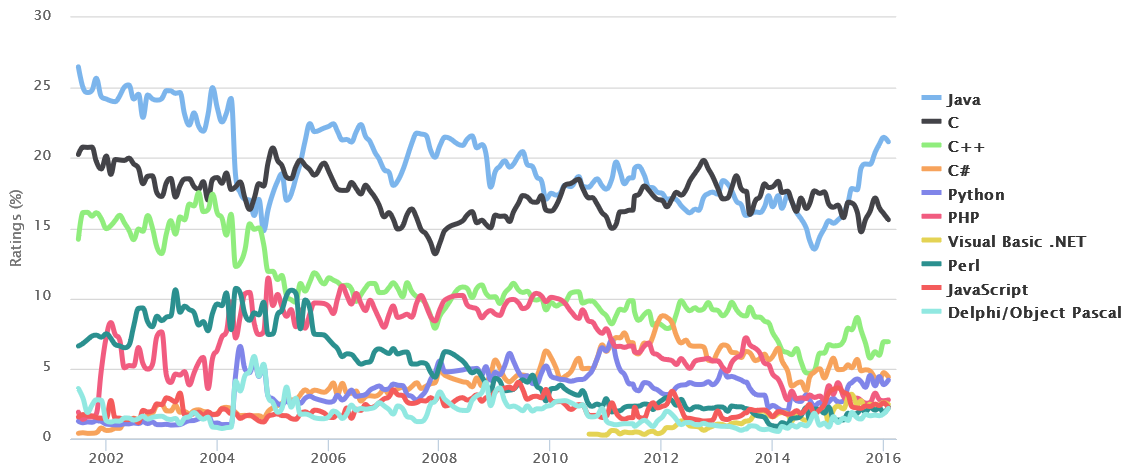
\includegraphics[keepaspectratio, width=\paperwidth]{images/LanguageTrend}
\end{figure}
}
\end{frame}
%
%-----------------------Frame 5-------------------------------
\placelogotrue
\placebackgroundfalse
%
\setbeamertemplate{background canvas}{
    \rule{0in}{3.5in}%
    \rule{0.53in}{0in}%
    \centering
    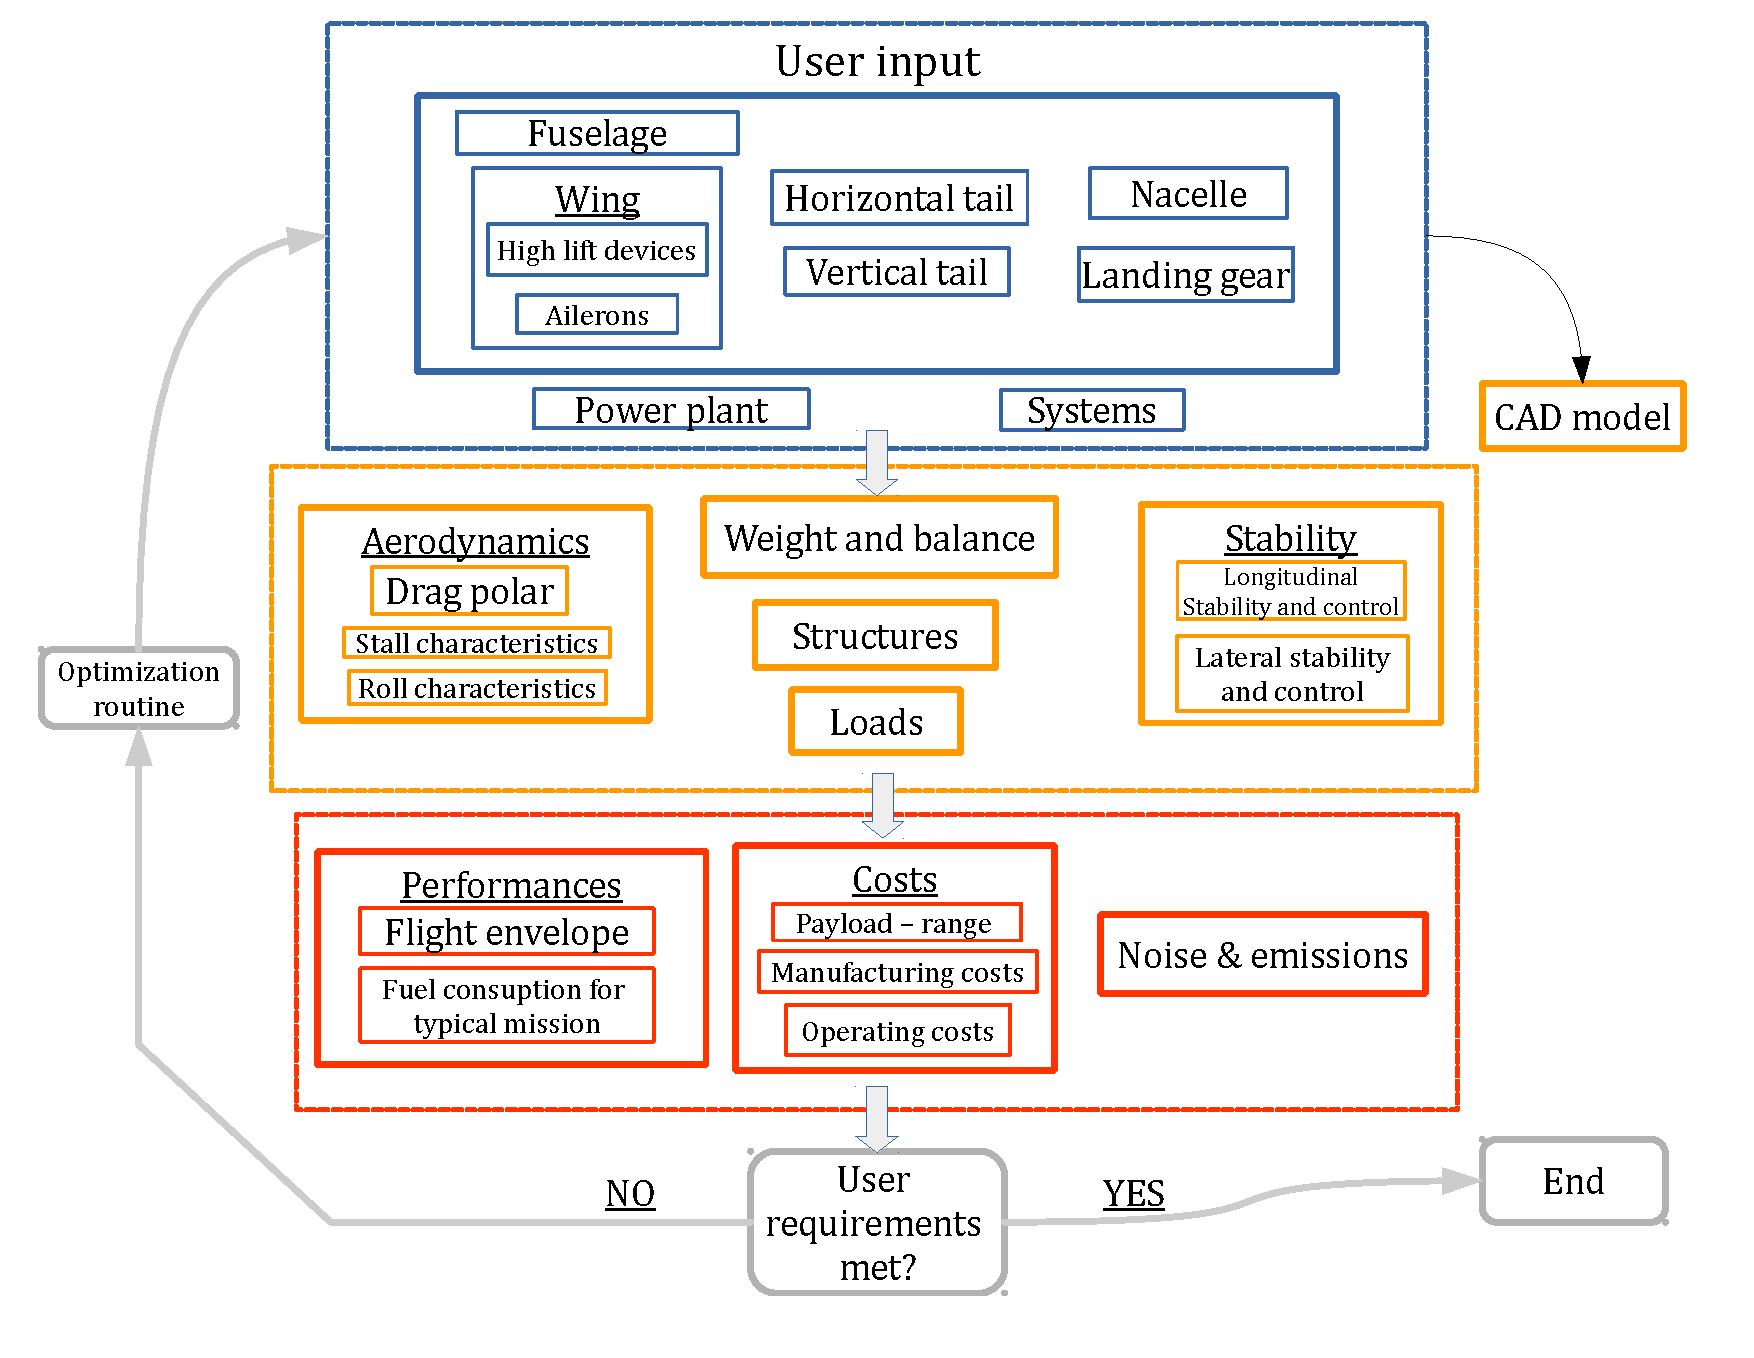
\includegraphics[keepaspectratio, width=0.73\paperwidth]{images/flowchart3}
}
%
\begin{frame}{JPAD typical work session}
\end{frame}
\setbeamertemplate{background canvas}{ }
%
%-----------------------Frame 6-------------------------------
\placelogotrue
\placebackgroundfalse
\begin{frame}{Input file}
\Wider{
The input file type chosen is the {\textcolor{mygold}{XML}} (\emph{{\textcolor{mygold}{eXtensible Markup Language}}}). It is a markup language that defines a set of rules for encoding documents in a format which is both \emph{{\textcolor{mygold}{human-readable}}} and \emph{{\textcolor{mygold}{machine-readable}}}; moreover its design goals of emphasize simplicity, generality and usability across the Internet.
%
\begin{itemize}
\MyBullet \emph{{\textcolor{mygold}{Markup Language}}} due to the use of tags that describes the content.
\MyBullet \emph{{\textcolor{mygold}{extensible}}} because the markup symbols are unlimited and self-defining, so that it is possible to use a personal tag for each data.
\end{itemize}
}
\end{frame}
%
%-----------------------Frame 7-------------------------------
\placelogotrue
\placebackgroundfalse
%
\setbeamertemplate{background canvas}{
    \rule{0in}{3.6in}%
    \rule{0.07in}{0in}%
    \centering
    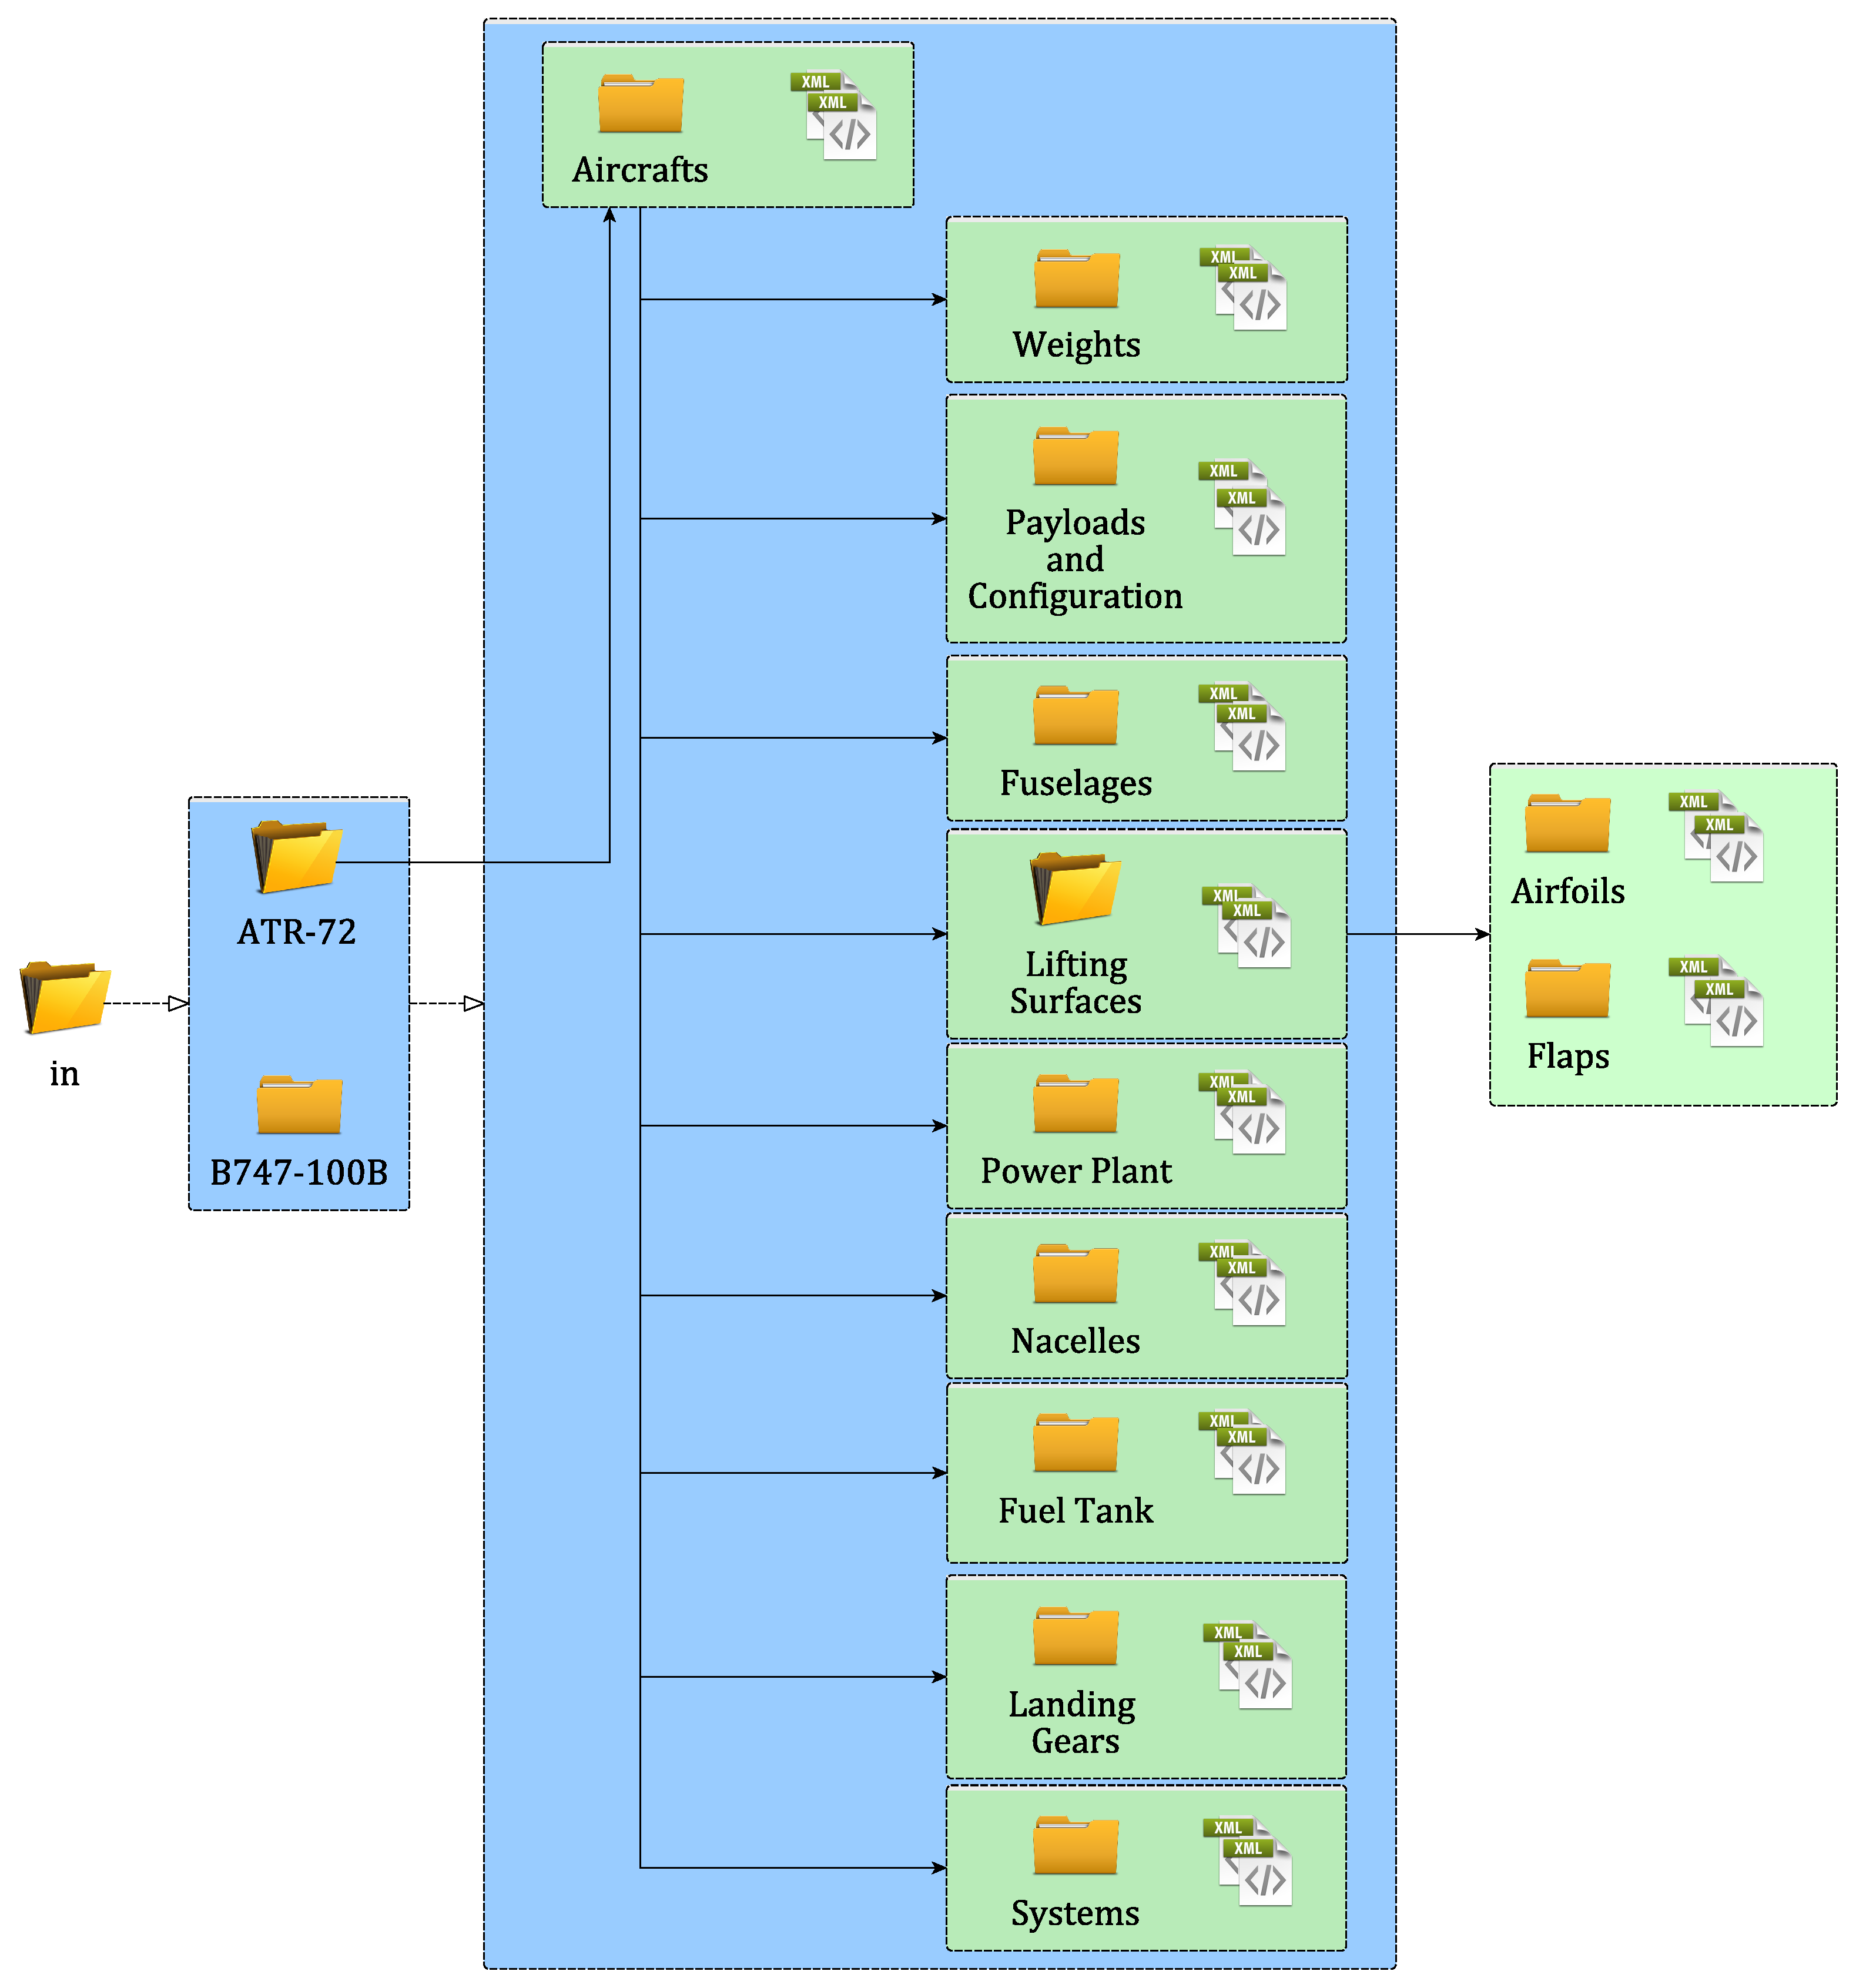
\includegraphics[keepaspectratio, width=0.55\paperwidth]{images/Folder_Tree}
}
%
\begin{frame}{Input file structure prototype}
\begin{figure}[!t]
    \hspace*{6.2cm}
    \vspace*{1.7cm}
    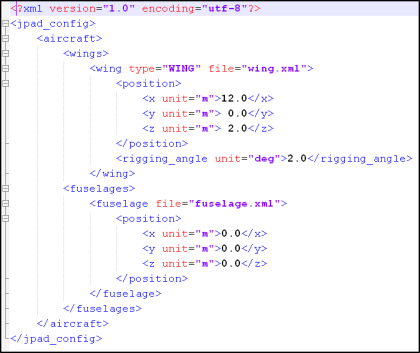
\includegraphics[keepaspectratio, width=0.415\paperwidth]{images/XMLAircraft}
\end{figure}
\end{frame}
\setbeamertemplate{background canvas}{ }
%
%-----------------------Frame 8-------------------------------
\placelogotrue
\placebackgroundfalse
%
\setbeamertemplate{background canvas}{
    \rule{0in}{2.775in}%
    \rule{2in}{0in}%
    \centering
    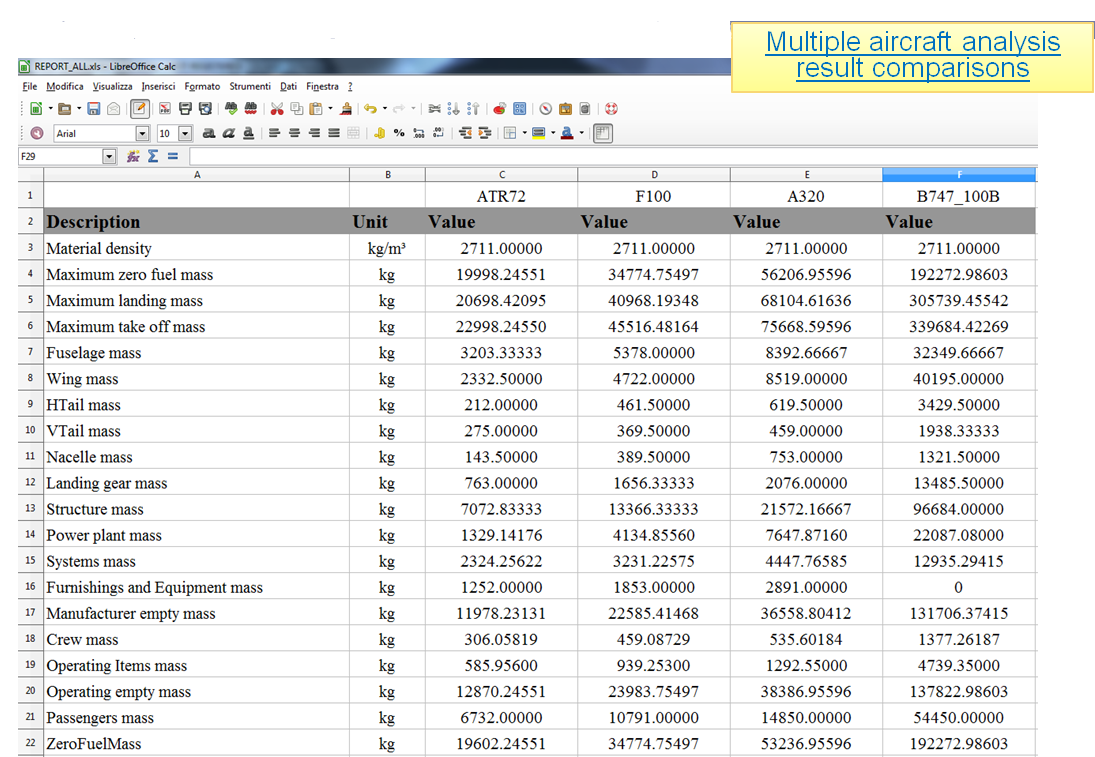
\includegraphics[keepaspectratio, width=0.6\paperwidth]{images/XLS}
}
%
\begin{frame}{JPAD Output}
\Wider{
\begin{itemize}
    \vspace*{-2cm}
\MyBullet XML
\MyBullet Microsoft Excel
\MyBullet Charts
\MyBullet CAD model
\end{itemize}
\begin{figure}[!t]
    \hspace*{-7.7cm}
    \vspace*{-3cm}
    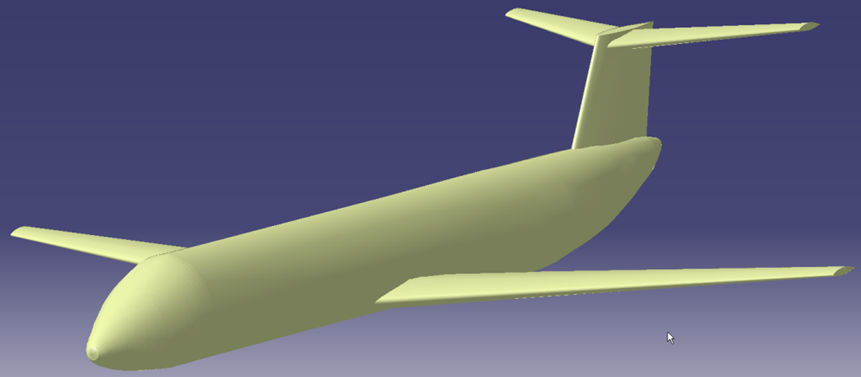
\includegraphics[keepaspectratio, width=0.4\paperwidth]{images/CAD}
\end{figure}
}
\end{frame}
%
\setbeamertemplate{background canvas}{}
%
%-----------------------Frame 9-------------------------------
\placelogotrue
\placebackgroundfalse
\begin{frame}{ADOpT GUI}
\Wider{
\begin{itemize}
	\MyBullet {\textcolor{mygold}{Menu bar}}, holds all the available actions.
	\MyBullet {\textcolor{mygold}{Toolbar}}, holds the actions needed to interact with the application.
	\MyBullet {\textcolor{mygold}{Project tree}}, provides access to all the aircraft components and the analysis results any time.
	\MyBullet {\textcolor{mygold}{3D view}}, shows the CAD model which can be updated each time.
	\MyBullet {\textcolor{mygold}{Log message window}}, tells the status of pending operations.
	\MyBullet {\textcolor{mygold}{Tab folder}}, contains all the windows opened.
\end{itemize}
}
\end{frame}
%
%-----------------------Frame 10-------------------------------
\placelogotrue
\placebackgroundfalse
%
\setbeamertemplate{background canvas}{
    \rule{0in}{3.12in}%
    \rule{0.1in}{0in}%
    \centering
    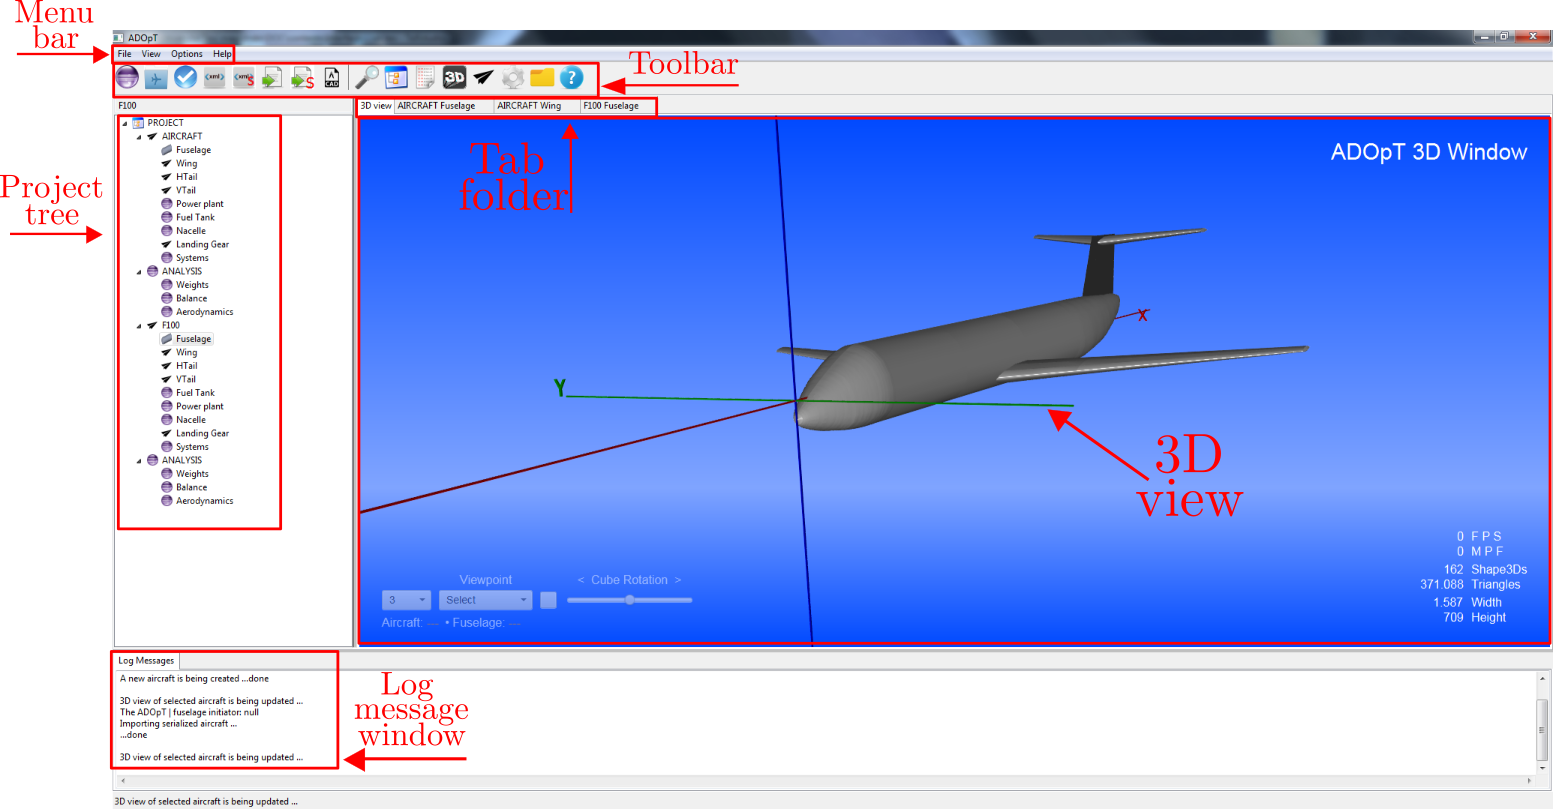
\includegraphics[keepaspectratio, width=0.95\paperwidth]{images/GUI}
}
%
\begin{frame}{ADOpT GUI - Layout}
\end{frame}
\setbeamertemplate{background canvas}{ }
%
%-----------------------Frame 11-------------------------------
\placelogotrue
\placebackgroundfalse
%
\setbeamertemplate{background canvas}{
    \rule{0in}{3.5in}%
    \rule{0.3in}{0in}%
    \centering
    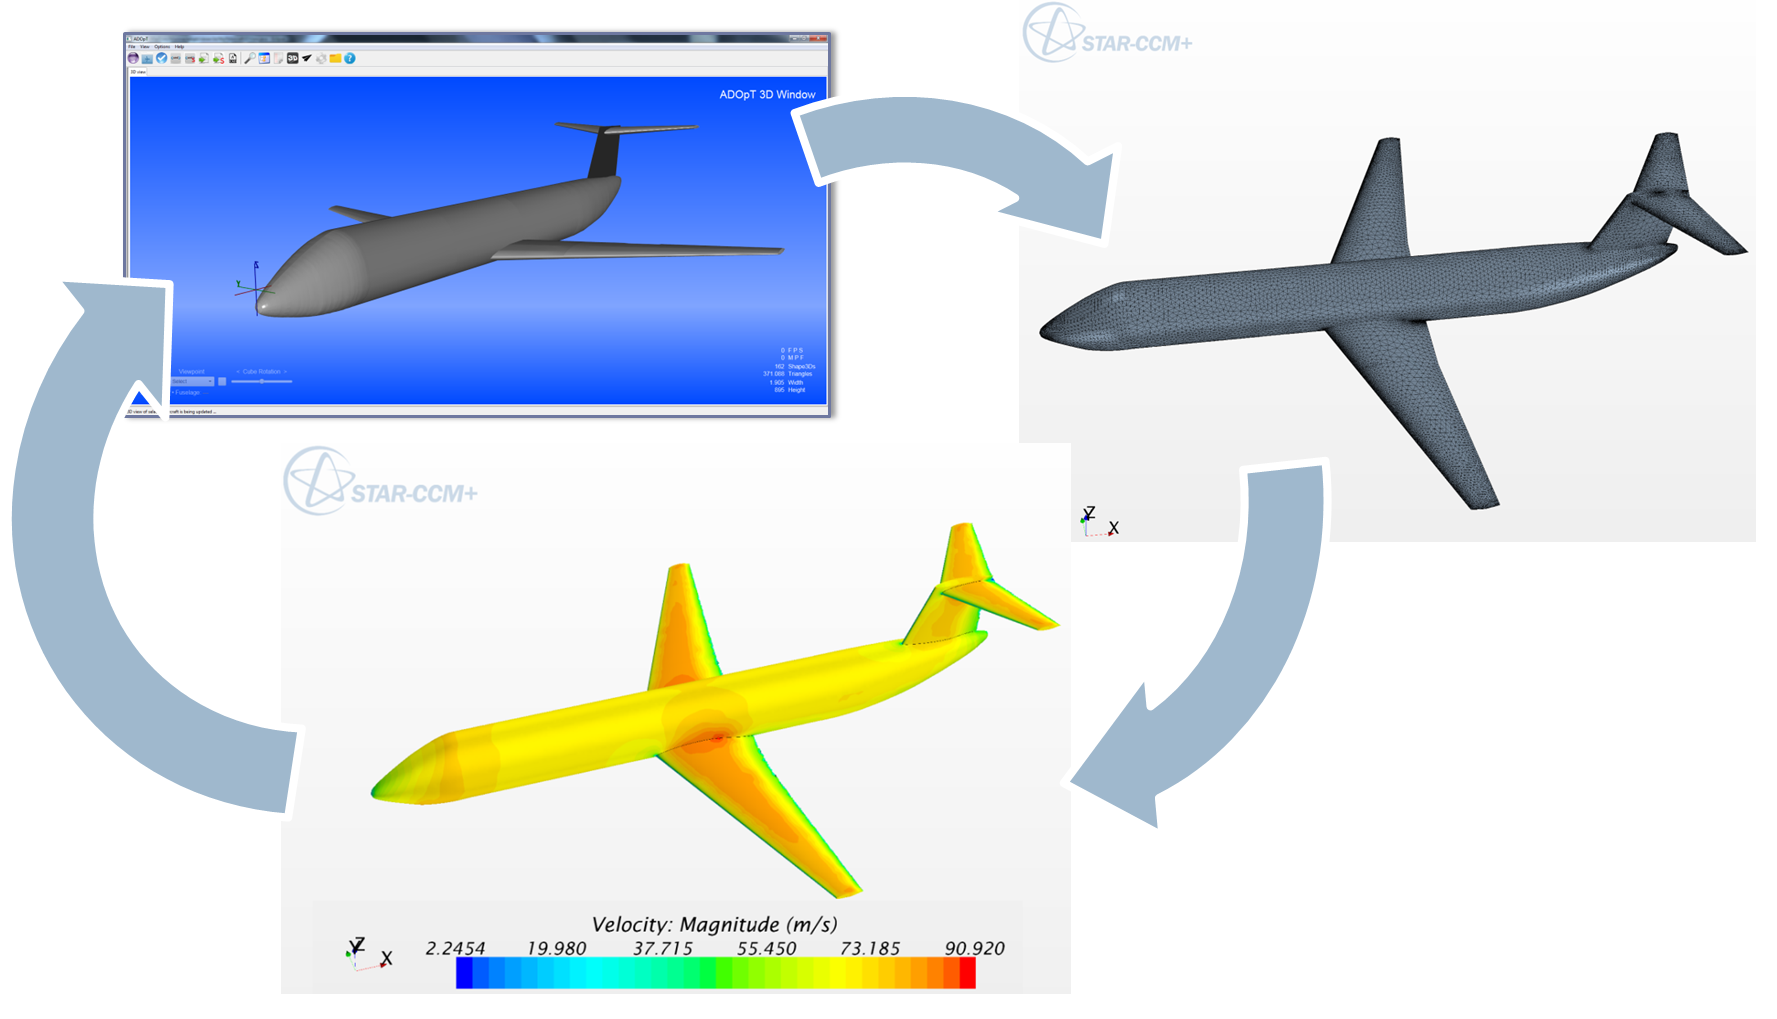
\includegraphics[keepaspectratio, width=0.94\paperwidth]{images/interface}
}
%
\begin{frame}{Interoperability}
\end{frame}
\setbeamertemplate{background canvas}{ }
%
%----------------Current table of contents--------------------
\placelogotrue
\placebackgroundfalse
\begin{frame}{Table of Contents}
\section{Payload Range class}
\vspace*{-1cm}
\tableofcontents[currentsection]
\subsection{}
\end{frame}
%
%-----------------------Frame 12-------------------------------
\placelogotrue
\placebackgroundfalse
\begin{frame}{Payload-Range chart construction}
\Wider{
\begin{columns}[onlytextwidth,t]
\column{0.6\textwidth}
\begin{itemize}
    \vspace*{0.5cm}
	\MyBullet {\textcolor{mygold}{Point A}}: Maximum payload at zero range. (\alert{Already known})
	\MyBullet {\textcolor{mygold}{Point B}}: Range at maximum payload and maximum take-off weight.
	\MyBullet {\textcolor{mygold}{Point C}}: Range at maximum take-off weight with maximum fuel in fuel tanks.
	\MyBullet {\textcolor{mygold}{Point D}}: Range with maximum fuel in fuel tanks and no payload.
\end{itemize}
\column{0.4\textwidth}
\begin{figure}[!t]
    \vspace*{-0.2cm}
    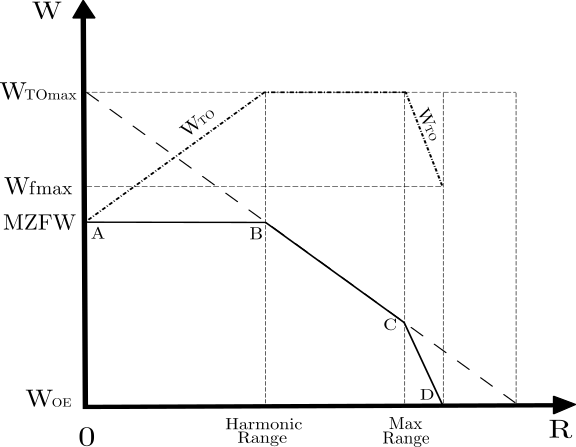
\includegraphics[keepaspectratio, width=0.4\paperwidth]{images/Payload_Range}
\end{figure}
\end{columns}
\begin{center}
    \vspace*{-0.35cm}
\begin{minipage}{4cm}
\begin{varblock}[6cm]{Breguet equation propeller aircraft}
\centering
\scalebox{0.8}{
$R=603.5\left(\frac{\eta_{p}}{SFC}\right)\left(\frac{L}{D}\right)\ln\left(\frac{W_{i}}{W_{f}}\right)_{\text{cruise}}$
}
\end{varblock}
%
\begin{varblock}[6cm]{Breguet equation jet aircraft}
\centering
\scalebox{0.8}{
$R=\left(\frac{V}{SFCJ}\right)\left(\frac{L}{D}\right)\ln\left(\frac{W_{i}}{W_{f}}\right)_{\text{cruise}}$
}
\end{varblock}
\end{minipage}
\end{center}
}
\end{frame}
%
%-----------------------Frame 13------------------------------
\placelogotrue
\placebackgroundfalse
\begin{frame}{Payload-Range chart construction}
\Wider{
\begin{itemize}
	\MyBullet {\textcolor{mygold}{Point B}}: $W_{TO,\text{max}}=W_{OE}+W_{\text{payload,max}}+\tikzmark{start1}W_{\text{fuel}}\tikzmark{end1}$
		
	\MyBullet {\textcolor{mygold}{Point C}}: $W_{TO,\text{max}}=W_{OE}+\tikzmark{start2}W_{\text{payload}}\tikzmark{end2}+W_{\text{fuel,max}}$
	\MyBullet {\textcolor{mygold}{Point D}}: $\tikzmark{start3}W_{\text{TO}}\tikzmark{end3}=W_{\text{OE}}+W_{\text{fuel,max}}$
		
\end{itemize}
\pause
\begin{tikzpicture}[remember picture,overlay]
\node[draw,line width=1pt,red,ellipse,inner ysep=7pt,fit={(pic cs:start1) (pic cs:end1)}] {};
\end{tikzpicture} 
\pause
\begin{tikzpicture}[remember picture,overlay]
\node[draw,line width=1pt,red,ellipse,inner ysep=7pt,fit={(pic cs:start2) (pic cs:end2)}] {};
\end{tikzpicture} 
\pause
\begin{tikzpicture}[remember picture,overlay]
\node[draw,line width=1pt,red,ellipse,inner ysep=7pt,fit={(pic cs:start3) (pic cs:end3)}] {};
\end{tikzpicture} 
\pause
\begin{itemize}
		\MyBullet $W_{\text{fuel}}=\left(1-M_{ff}\right)\cdot W_{TO}$
		\MyBullet $M_{ff}=\frac{W_1}{W_{TO}}\cdot 
	   		\frac{W_2}{W_{1}}\cdot
			   \frac{W_3}{W_{2}}\cdot 
			   \frac{W_4}{W_{3}}\cdot 
			   {\textcolor{mygold}{\frac{W_5}{W_{4}}}}\cdot 
			   \frac{W_6}{W_{5}}\cdot 
			   \frac{W_7}{W_{6}}\cdot 
			   \frac{W_8}{W_{7}}\cdot 
			   \frac{W_9}{W_{8}}\cdot 
			   \frac{W_{10}}{W_{9}}\cdot 
			   \frac{W_{\text{final}}}{W_{10}}$
\end{itemize}
\pause
\bigskip
\begin{itemize}
	\MyBullet For each point the couple Range-Payload can be calculated, where the payload for {\textcolor{mygold}{point C}} is obtained from the previous equations.
\end{itemize}
}
\end{frame}
%
%-----------------------Frame 14------------------------------
\placelogotrue
\placebackgroundfalse
\begin{frame}{Payload-Range Java class flowchart}
\WiderImages{
\only<1>{
\begin{figure}
\centering
    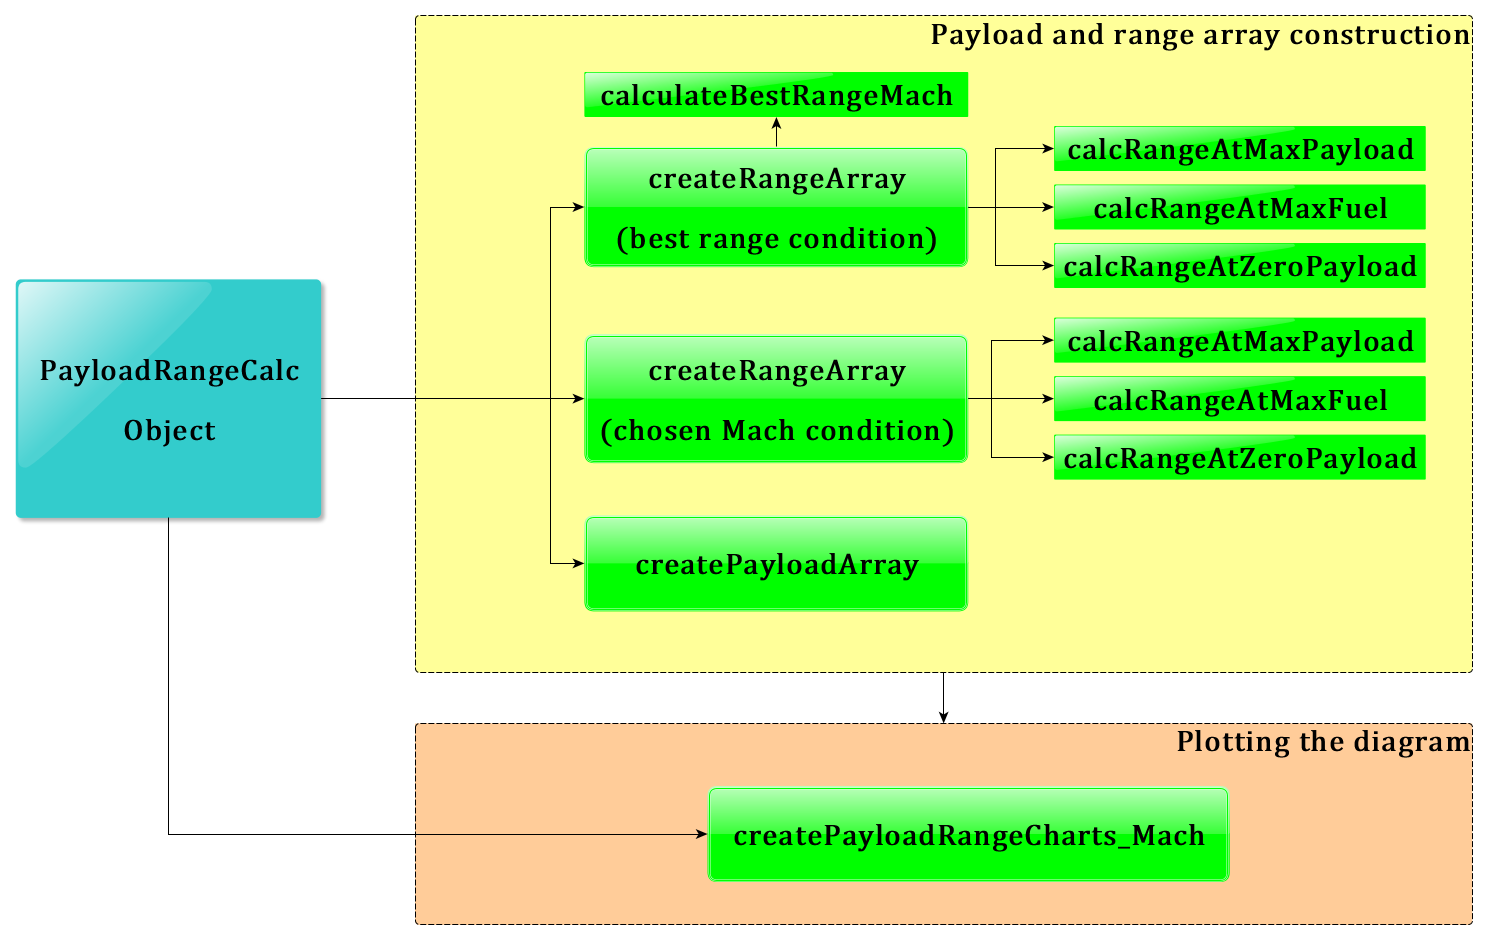
\includegraphics[keepaspectratio, width=0.73\paperwidth]{images/PayloadRange_BestRange_Flowchart.png}
    \captionsetup{labelformat=empty}
    \caption{\scalebox{0.8}{\qquad\qquad\qquad \textbf{Flowchart for best range and chosen Mach conditions comparison}}}
\end{figure}
}
\only<2>{
\begin{figure}
\centering
    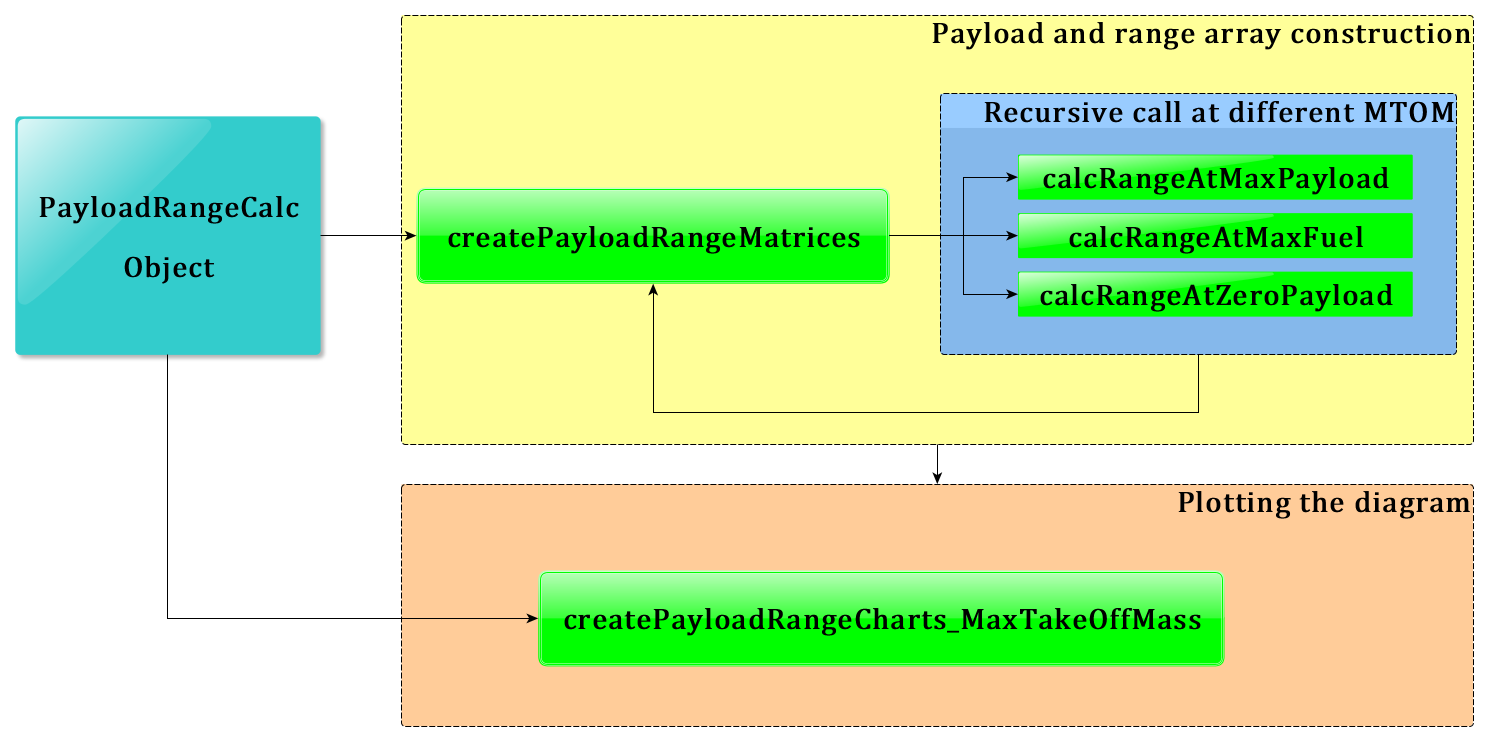
\includegraphics[keepaspectratio, width=0.8\paperwidth]{images/PayloadRange_MTOM_Flowchart.png}
    \captionsetup{labelformat=empty}
    \caption{\scalebox{0.8}{\qquad\qquad\qquad\qquad\qquad \textbf{Flowchart for maximum take-off mass parameterization}}}
\end{figure}
}
}
\end{frame}
%
%-----------------------Frame 15------------------------------
\placelogotrue
\placebackgroundfalse
\begin{frame}{Payload-Range Java class output}
\Wider{
  \vspace*{0.1cm}
  \hspace*{0.9cm}
\scalebox{0.8}{
\begin{tabular}{|l||c|c|c|c|c|}
\hline
\textbf{ } & \textbf{ATR-72} &\textbf{ } &  \textbf{JPAD} &\textbf{ } & \textbf{Difference(\%)}\\
\hline\hline
\textbf{Range} & 890 nmi  & \textbf{ } &$\approx820$ nmi &\textbf{ } & $\approx7.8$\%\\
\textbf{Payload} & 68 pass. at $\SI{95}{\kilogram}$ &\textbf{ } & 65 pass. at $\SI{99}{\kilogram}$ &\textbf{ } & \textbf{ }\\
\hline
\end{tabular}
}
}
\WiderImages{
\begin{columns}[onlytextwidth,t]
\column{0.5\textwidth}
\begin{figure}
  \vspace*{-0.9cm}
\centering
    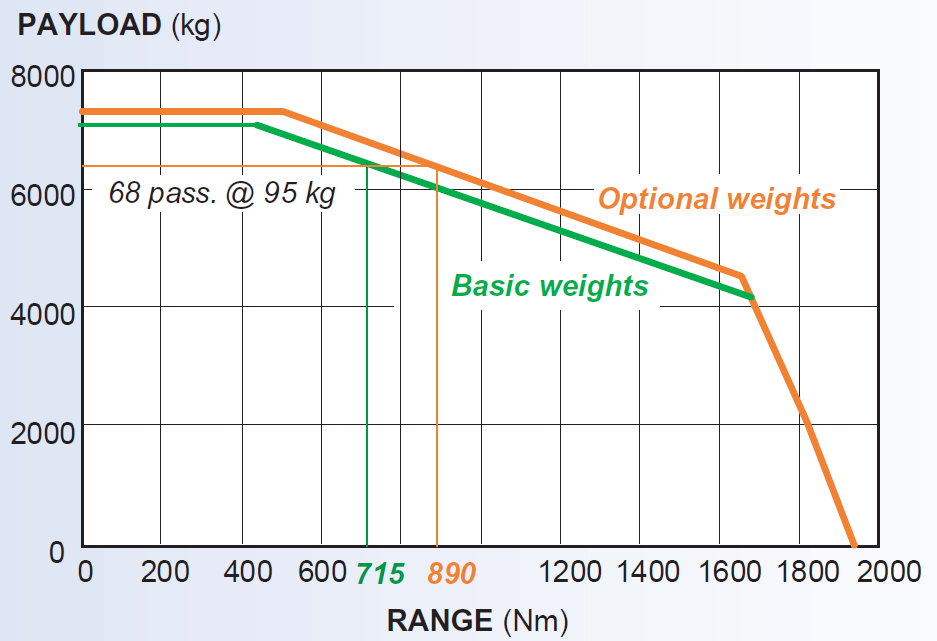
\includegraphics[keepaspectratio, width=0.5\paperwidth]{images/ATRSpecsPR.PNG}
    \captionsetup{labelformat=empty}
    \caption{\scalebox{0.7}{\qquad\qquad \textbf{ATR 72-500 data} (MTOM optional $\SI{22800}{\kilogram}$)}}
\end{figure}
\column{0.5\textwidth}
\begin{figure}
  \vspace*{-0.8cm}
\centering
    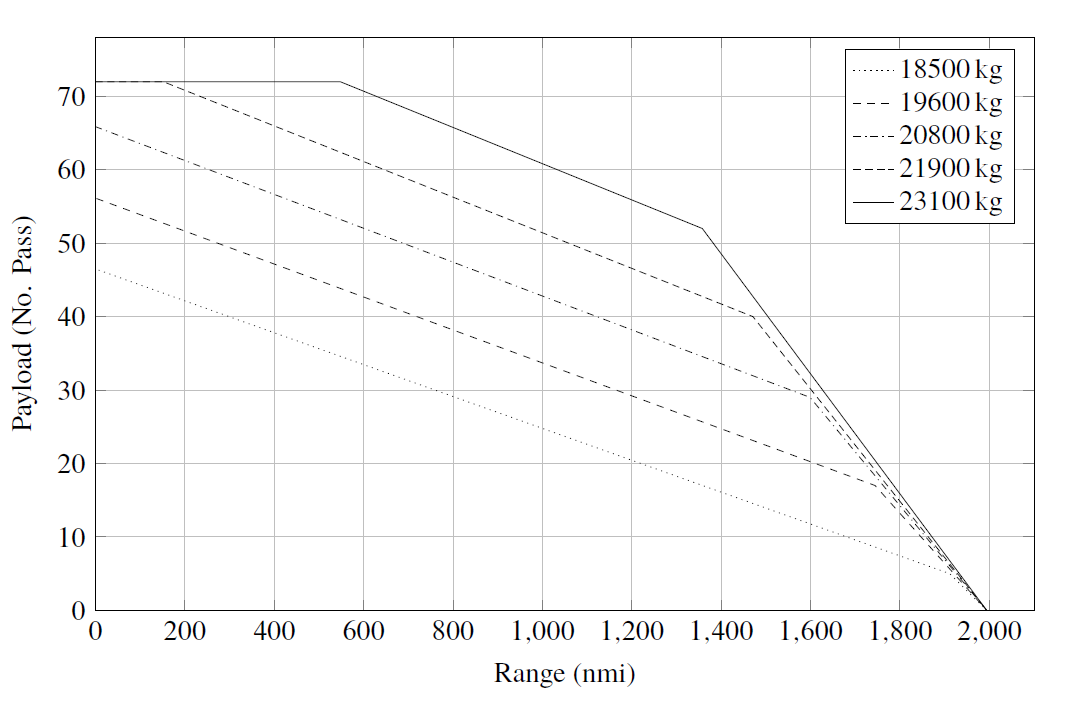
\includegraphics[keepaspectratio, width=0.5\paperwidth]{images/ATRJpadPR.PNG}
    \captionsetup{labelformat=empty}
\end{figure}
\end{columns}
}
\end{frame}
%
%-----------------------Frame 16------------------------------
\placelogotrue
\placebackgroundfalse
\begin{frame}{Payload-Range Java class output}
\Wider{
  \vspace*{-0.25cm}
  \hspace*{0.9cm}
\scalebox{0.8}{
\begin{tabular}{|l||c|c|c|c|c|}
\hline
\textbf{ } & \textbf{B747-100B} &\textbf{ } &  \textbf{JPAD} &\textbf{ } & \textbf{Difference(\%)}\\
\hline\hline
\textbf{Range} & $\approx5200$ nmi &\textbf{ } & $\approx5300$ nmi &\textbf{ } & $\approx1.9$\%\\
\textbf{Payload} & 452 pass. at $\SI{95}{\kilogram}$ &\textbf{ } & 434 pass. at $\SI{99}{\kilogram}$ &\textbf{ } & \textbf{ }\\
\hline
\end{tabular}
}
}
\WiderImages{
\begin{columns}[onlytextwidth,t]
\column{0.5\textwidth}
\begin{figure}
  \vspace*{-0.4cm}
\centering
    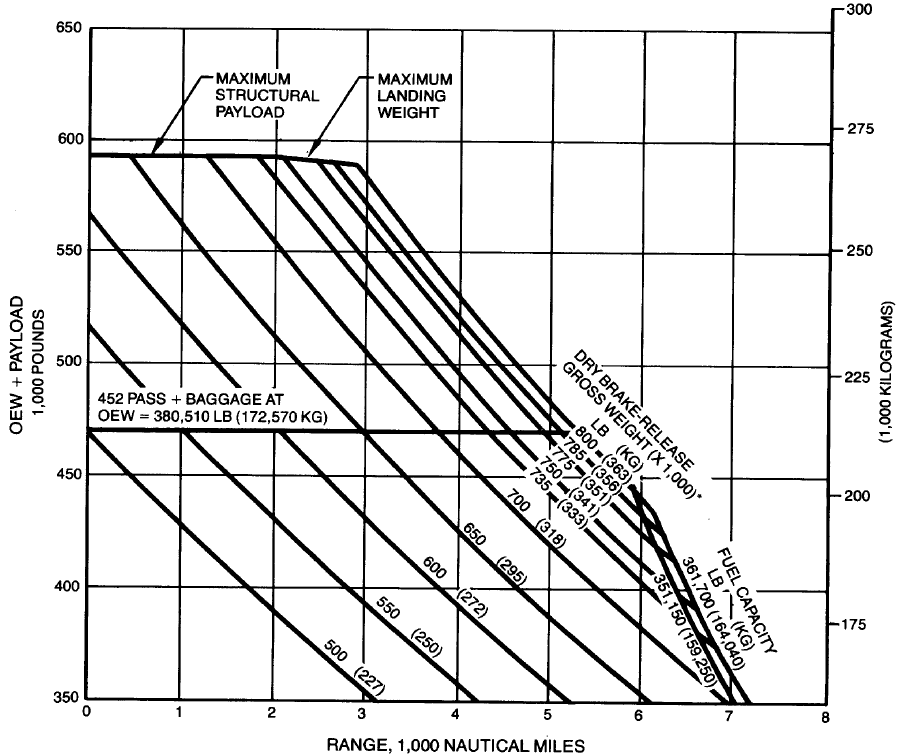
\includegraphics[keepaspectratio, width=0.47\paperwidth]{images/B747SpecsPR.PNG}
    \captionsetup{labelformat=empty}
\end{figure}
\column{0.5\textwidth}
\begin{figure}
  \vspace*{-0.3cm}
\centering
    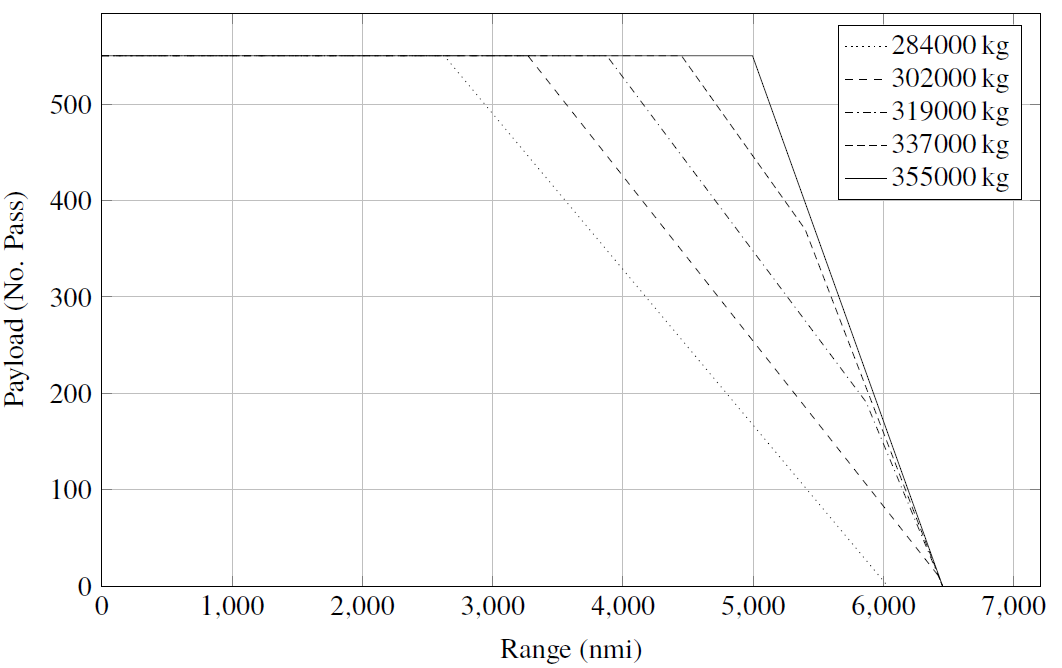
\includegraphics[keepaspectratio, width=0.5\paperwidth]{images/B747JpadPR.PNG}
    \captionsetup{labelformat=empty}
\end{figure}
\end{columns}
}
\end{frame}
%----------------Current table of contents--------------------
\placelogotrue
\placebackgroundfalse
\begin{frame}{Table of Contents}
\section{Specific Range class}
\vspace*{-1cm}
\tableofcontents[currentsection]
\subsection{}
\end{frame}
%
%-----------------------Frame 17------------------------------
\placelogotrue
\placebackgroundfalse
\begin{frame}{Specific Range and Cruise Grid chart}
\Wider{
\begin{columns}[onlytextwidth,t]
\column{0.6\textwidth}
\begin{itemize}
    \vspace*{0.6cm}
	\MyBullet {\textcolor{mygold}{Cruise grid chart}} is a very important tool for pilots because it allows to choose the correct speed, during the cruise phase, in order to follow some mission objectives like minimum fuel consumption or a fast cruise.
	\MyBullet In {\textcolor{mygold}{Breguet equations}} the focus is on the {\textcolor{mygold}{autonomy factor A.F.}}.
\end{itemize}
\column{0.4\textwidth}
\begin{figure}[!t]
    \vspace*{-0.2cm}
    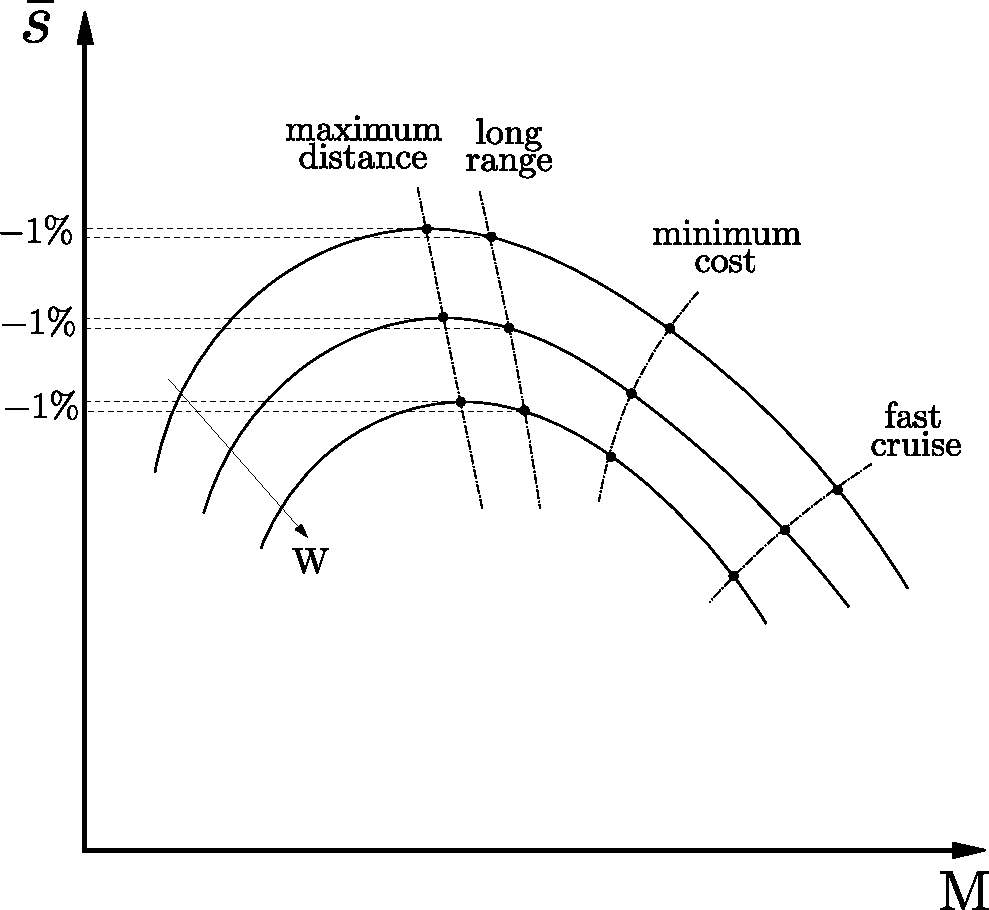
\includegraphics[keepaspectratio, width=0.4\paperwidth]{images/CruiseGrid}
\end{figure}
\end{columns}
%
\begin{center}
 \vspace*{-0.65cm}
\begin{minipage}{4cm}
\begin{varblock}[4cm]{Autonomy Factor Propeller}
\centering
\scalebox{0.8}{
$A.F.=\left(\frac{\eta_{p}}{SFC}\right)\left(\frac{L}{D}\right)$ 
}
\end{varblock}
%
\begin{varblock}[4cm]{Autonomy Factor Jet}
\centering
\scalebox{0.8}{
$A.F.=\left(\frac{V}{SFCJ}\right)\left(\frac{L}{D}\right)$
}
\end{varblock}
\end{minipage}
\end{center}
}
\end{frame}
%
%-----------------------Frame 18------------------------------
\placelogotrue
\placebackgroundfalse
\begin{frame}{Specific Range calculation}
\Wider{
\begin{itemize}
        \MyBullet From the aircraft weight in cruise condition the {\textcolor{mygold}{$C_L$}} can be calculated.
        \MyBullet With this $C_L$ the related {\textcolor{mygold}{$C_D$}} can be calculated taking into account the wave drag, if present.
        \MyBullet From engine database the {\textcolor{mygold}{SFC}} can be easily calculated in the given flight condition.
        \MyBullet At a given speed, or with known propeller efficiency, the {\textcolor{mygold}{A.F.}} can be calculated.
	\MyBullet The {\textcolor{mygold}{specific range}} can be calculated from the {\textcolor{mygold}{A.F. dividing it by the aircraft weight}} in cruise.
	\MyBullet This can be done for {\textcolor{mygold}{several Mach numbers}}, between the maximum and minimum one from the flight envelope at that altitude, and {\textcolor{mygold}{several aircraft weights}}.
\end{itemize}
}
\end{frame}
%
%-----------------------Frame 19------------------------------
\placelogotrue
\placebackgroundfalse
%
\setbeamertemplate{background canvas}{
    \rule{0in}{3.12in}%
    \rule{0.3in}{0in}%
    \centering
    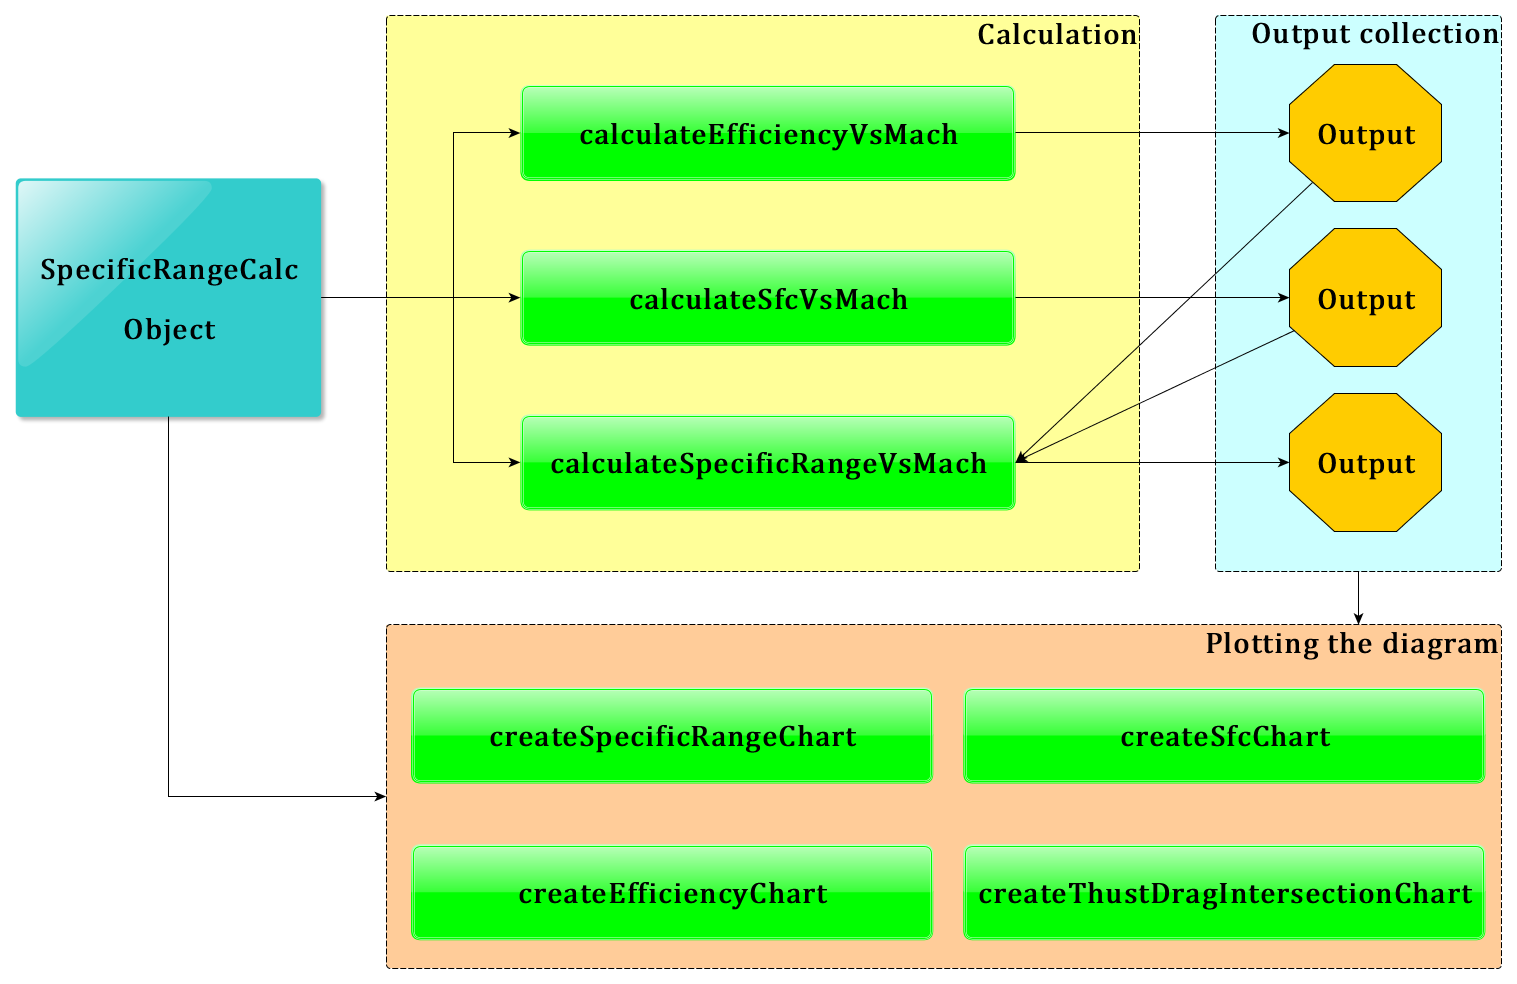
\includegraphics[keepaspectratio, width=0.75\paperwidth]{images/SpecificRange_Flowchart.png}
}
%
\begin{frame}{Specific Range Java class flowchart}
\end{frame}
\setbeamertemplate{background canvas}{ }
%
%-----------------------Frame 20------------------------------
\placelogotrue
\placebackgroundfalse
%
\setbeamertemplate{background canvas}{
    \rule{0in}{2.7in}%
    \rule{3.8in}{0in}%
    \centering
    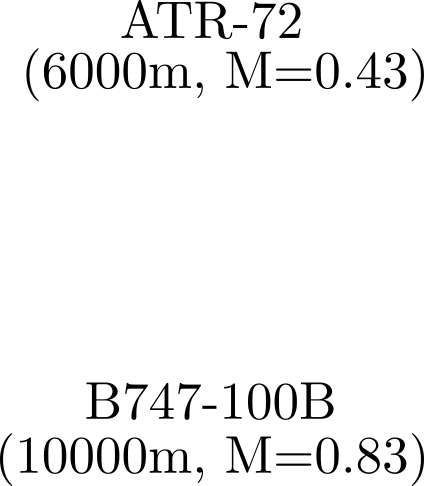
\includegraphics[keepaspectratio, width=0.23\paperwidth]{images/ATRB747CruiseCond.png}
}
%
\begin{frame}{Specific Range Java class output}
\only<1>{
\WiderImages{
\begin{figure}
  \vspace*{0.42cm}
    \hspace*{-0.7cm}
\centering
    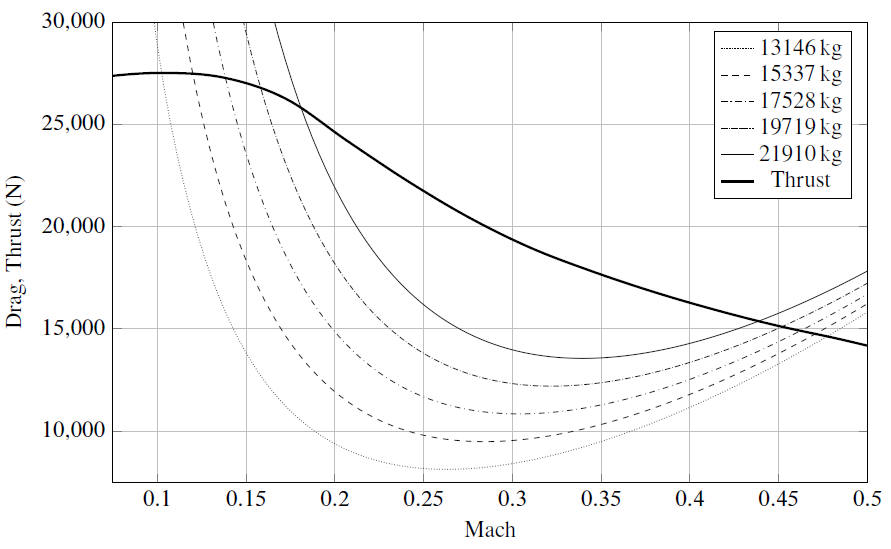
\includegraphics[keepaspectratio, width=0.5\paperwidth]{images/DragThrustATR.PNG}
    \captionsetup{labelformat=empty}
\end{figure}
\begin{figure}
  \vspace*{-1.15cm}
  \hspace*{-0.7cm}
\centering
    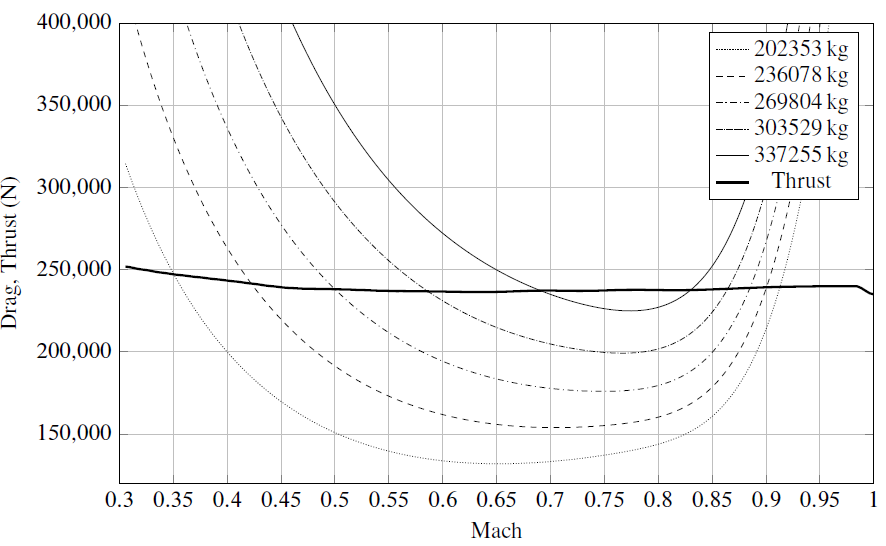
\includegraphics[keepaspectratio, width=0.5\paperwidth]{images/DragThrustB747.PNG}
    \captionsetup{labelformat=empty}
\end{figure}
}
}
\pause
\only<2>{
\WiderImages{
\begin{figure}
  \vspace*{0.38cm}
    \hspace*{-0.2cm}
\centering
    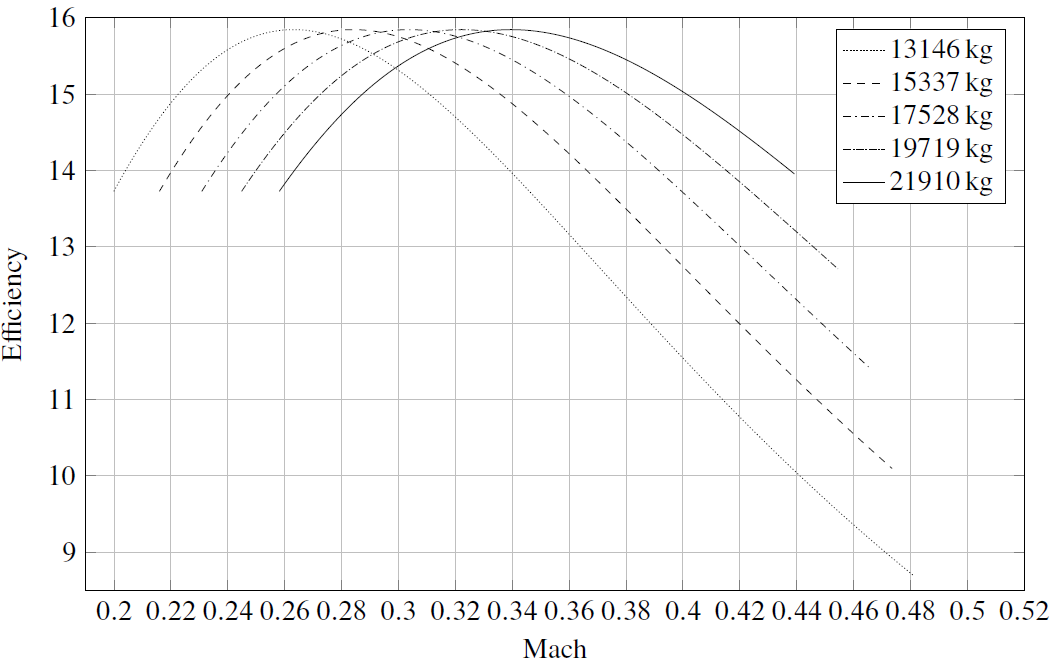
\includegraphics[keepaspectratio, width=0.495\paperwidth]{images/EfficiencyATR.PNG}
    \captionsetup{labelformat=empty}
\end{figure}
\begin{figure}
  \vspace*{-1.14cm}
  \hspace*{-0.2cm}
\centering
    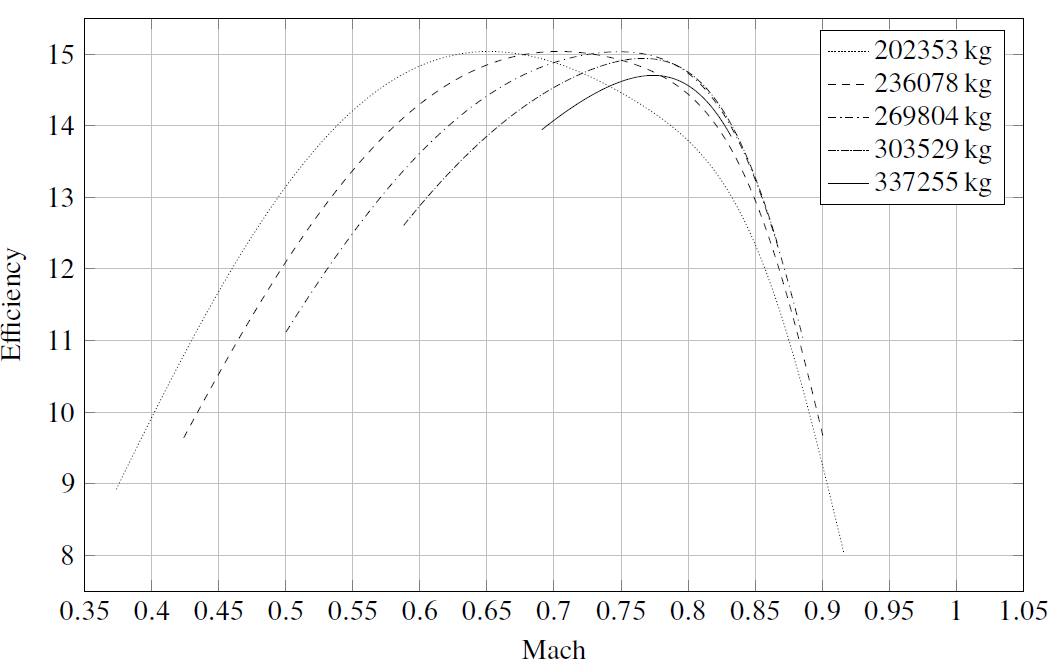
\includegraphics[keepaspectratio, width=0.495\paperwidth]{images/EfficiencyB747.PNG}
    \captionsetup{labelformat=empty}
\end{figure}
}
}
\pause
\only<3>{
\WiderImages{
\begin{figure}
  \vspace*{0.38cm}
    \hspace*{-0.2cm}
\centering
    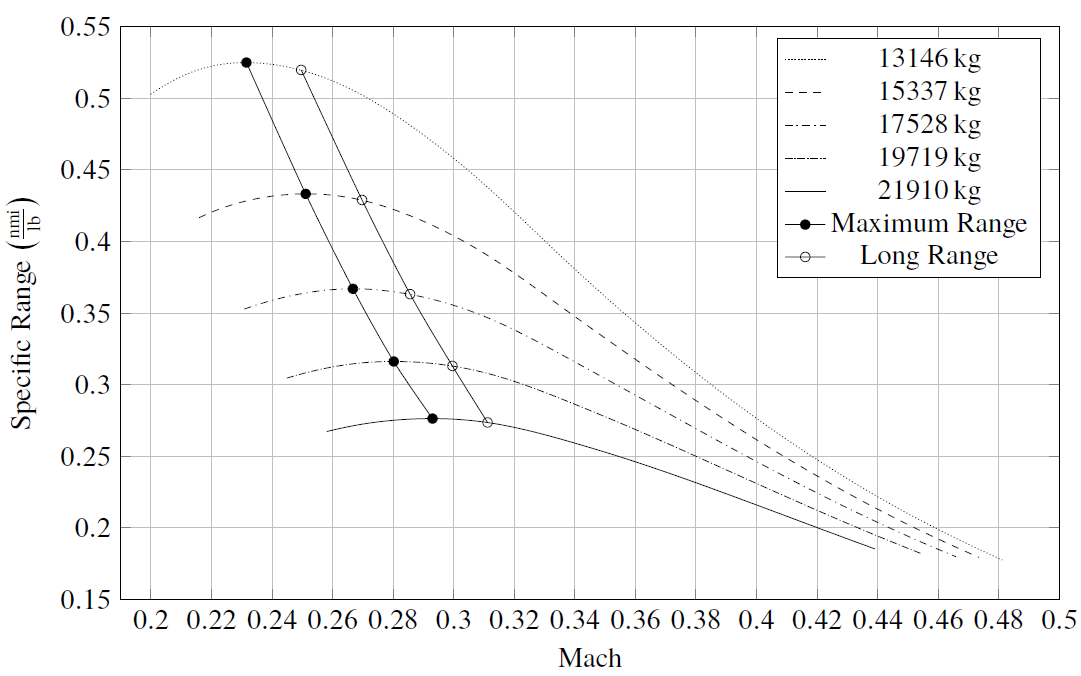
\includegraphics[keepaspectratio, width=0.5\paperwidth]{images/CruiseGridATR.PNG}
    \captionsetup{labelformat=empty}
\end{figure}
\begin{figure}
  \vspace*{-1.08cm}
  \hspace*{-0.2cm}
\centering
    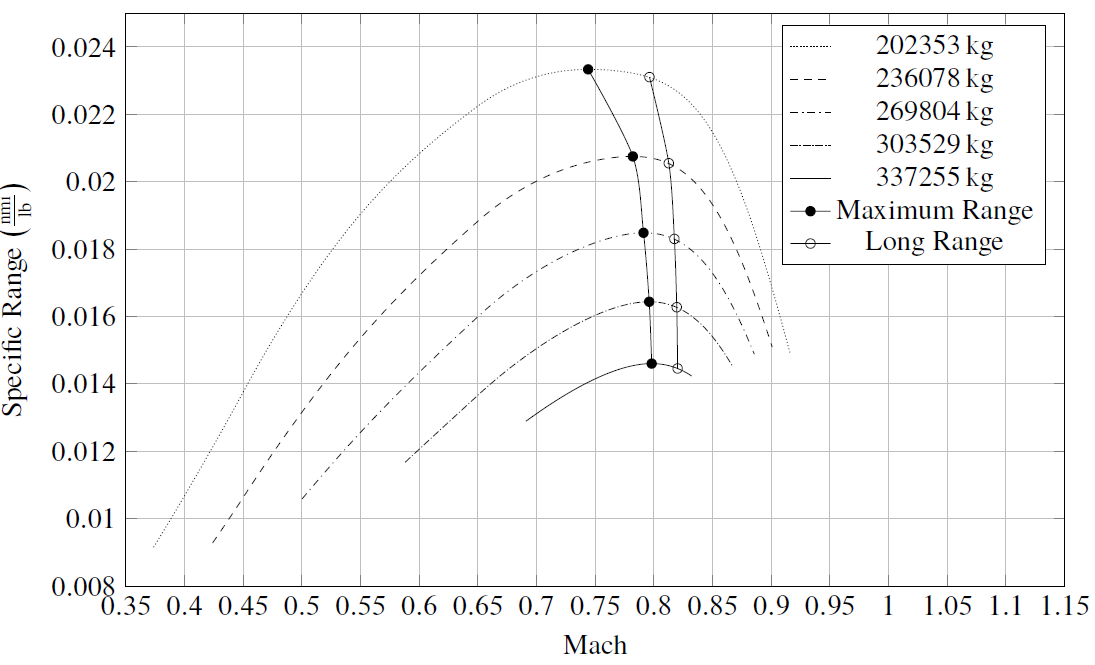
\includegraphics[keepaspectratio, width=0.51\paperwidth]{images/CruiseGridB747.PNG}
    \captionsetup{labelformat=empty}
\end{figure}
}
}
\end{frame}
\setbeamertemplate{background canvas}{ }
%
%----------------Current table of contents--------------------
\placelogotrue
\placebackgroundfalse
\begin{frame}{Table of Contents}
\section{High Lift Devices class}
\vspace*{-1cm}
\tableofcontents[currentsection]
\subsection{}
\end{frame}
%
%-----------------------Frame 21------------------------------
\placelogotrue
\placebackgroundfalse
\begin{frame}{Trailing-edge devices effects}
\Wider{
\begin{columns}[onlytextwidth,t]
\column{0.5\textwidth}
	\begin{itemize}
	\vspace*{0.8cm}
	\MyBullet Higher $C_L$ at a given angle of attack and higher $C_{\text{Lmax}}$.
	\MyBullet Lower stalling angle of attack.
	\MyBullet Lower zero-lift angle due to increasing camber.
	\end{itemize}
\begin{figure}
	\vspace*{0.3cm}
	\hspace*{-0.2cm}
	\centering
	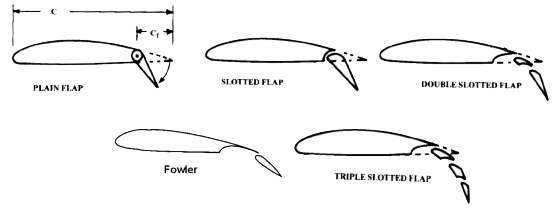
\includegraphics[keepaspectratio, width=0.6\paperwidth]{images/Flap}
\end{figure}
\column{0.5\textwidth}
	\begin{figure}
	\vspace*{-0.4cm}
	\hspace*{0.55cm}
	\centering
    	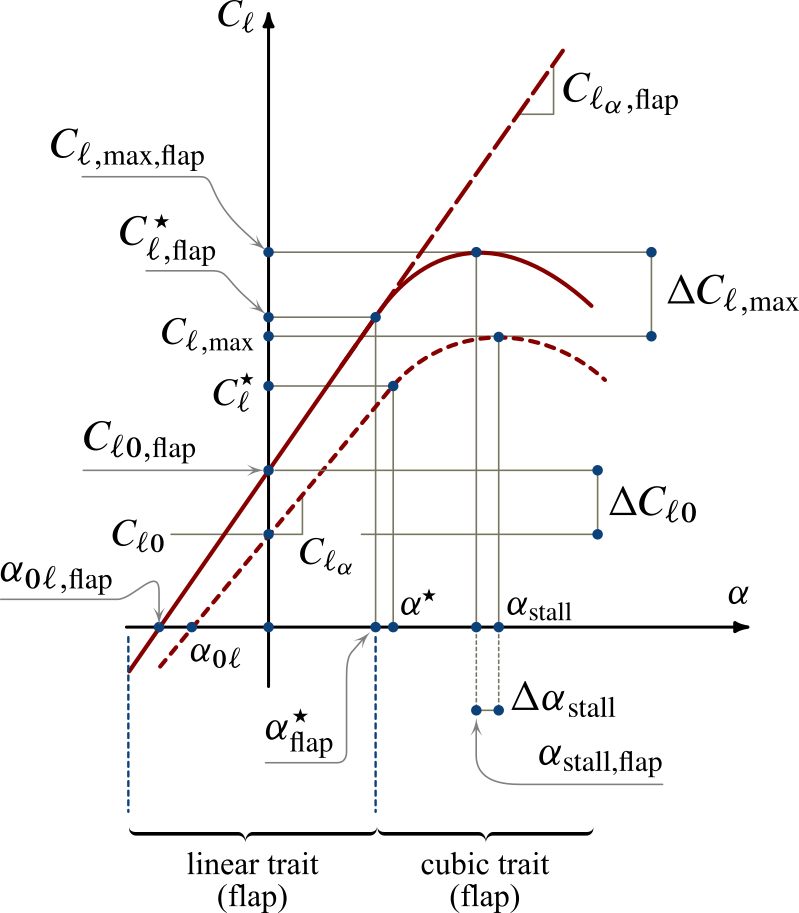
\includegraphics[keepaspectratio, width=0.445\paperwidth]{images/FlapEffects}
\end{figure}
\end{columns}
}
\end{frame}
%
%-----------------------Frame 22------------------------------
\placelogotrue
\placebackgroundfalse
\begin{frame}{Leading-edge devices effects}
\Wider{
\begin{columns}[onlytextwidth,t]
\column{0.5\textwidth}
	\begin{itemize}
	\vspace*{0.8cm}
	\MyBullet Extension of the linear trait of the lift curve with an increase of the stalling angle of attack and of the $C_{\text{Lmax}}$
	\MyBullet Higher zero-lift angle caused by leading edge deflection which reduce the actual angle of attack.
	\MyBullet Higher slope of the linear trait of the lift curve.
	\end{itemize}
\begin{figure}
	\vspace*{-0.6cm}
	\hspace*{1.8cm}
	\centering
	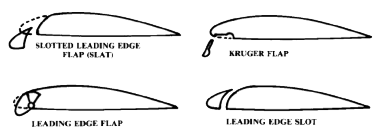
\includegraphics[keepaspectratio, width=0.46\paperwidth]{images/Slat}
\end{figure}
\column{0.5\textwidth}
	\begin{figure}
	\vspace*{-0.1cm}
	\hspace*{0.45cm}
	\centering
    	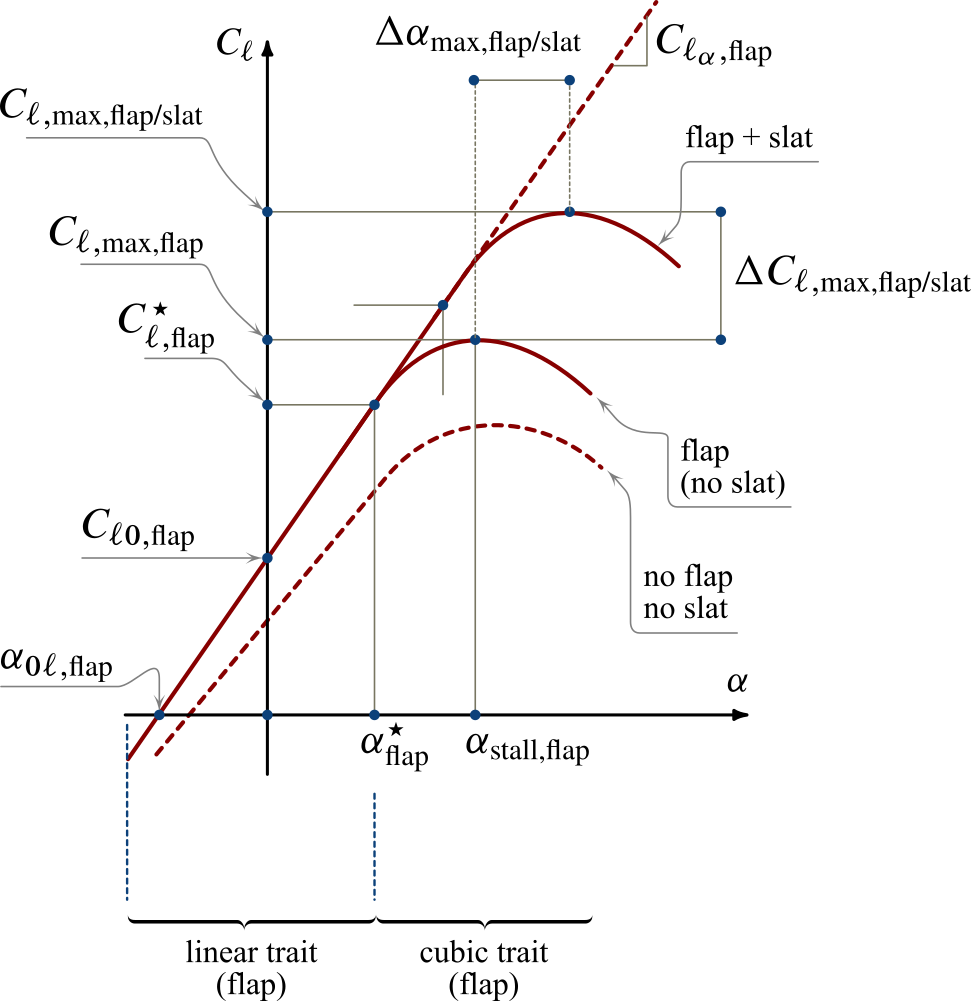
\includegraphics[keepaspectratio, width=0.45\paperwidth]{images/SlatEffects}
\end{figure}
\end{columns}
}
\end{frame}
%
%-----------------------Frame 23------------------------------
\placelogotrue
\placebackgroundfalse
\begin{frame}{Calculation methodologies}
\Wider{
\begin{itemize}
	\MyBullet Charts, semi-empirical equations and experimental data have been used to evaluate high lift devices effects. (e.g.: \emph{Glauert’s linearized theory for thin airfoils with flaps, DATCOM, Young and Hufton experimental data})
\end{itemize}
\begin{itemize}
	\MyBullet Effects to evaluate:
	\begin{itemize}
		\MyBullet  \textbf{{\textcolor{mygold}{\text{$\Delta$}$C_{l0}$, \text{$\Delta$}$C_{L0}$}}}
		\MyBullet  \textbf{{\textcolor{mygold}{\text{$\Delta$}$C_{l\text{max}}$, \text{$\Delta$}$C_{L\text{max}}$}}}
		\MyBullet   \textbf{{\textcolor{mygold}{$C_{L\alpha, \text{flap}}$}}}
		\MyBullet  \textbf{{\textcolor{mygold}{\text{$\Delta$}$\alpha_{\text{stall,airfoil}}$, \text{$\Delta$}$\alpha_{\text{stall,wing}}$}}}
		\MyBullet  \textbf{{\textcolor{mygold}{\text{$\Delta$}$C_{D\text{0}}$}}}
		\MyBullet  \textbf{{\textcolor{mygold}{\text{$\Delta$}$C_{M\text{, c/4}}$}}}
	\end{itemize}
\end{itemize}
}
\end{frame}
%
%-----------------------Frame 24------------------------------
\placelogotrue
\placebackgroundfalse
%
\setbeamertemplate{background canvas}{
    \rule{0in}{3.6in}%
    \rule{0.19in}{0in}%
    \centering
    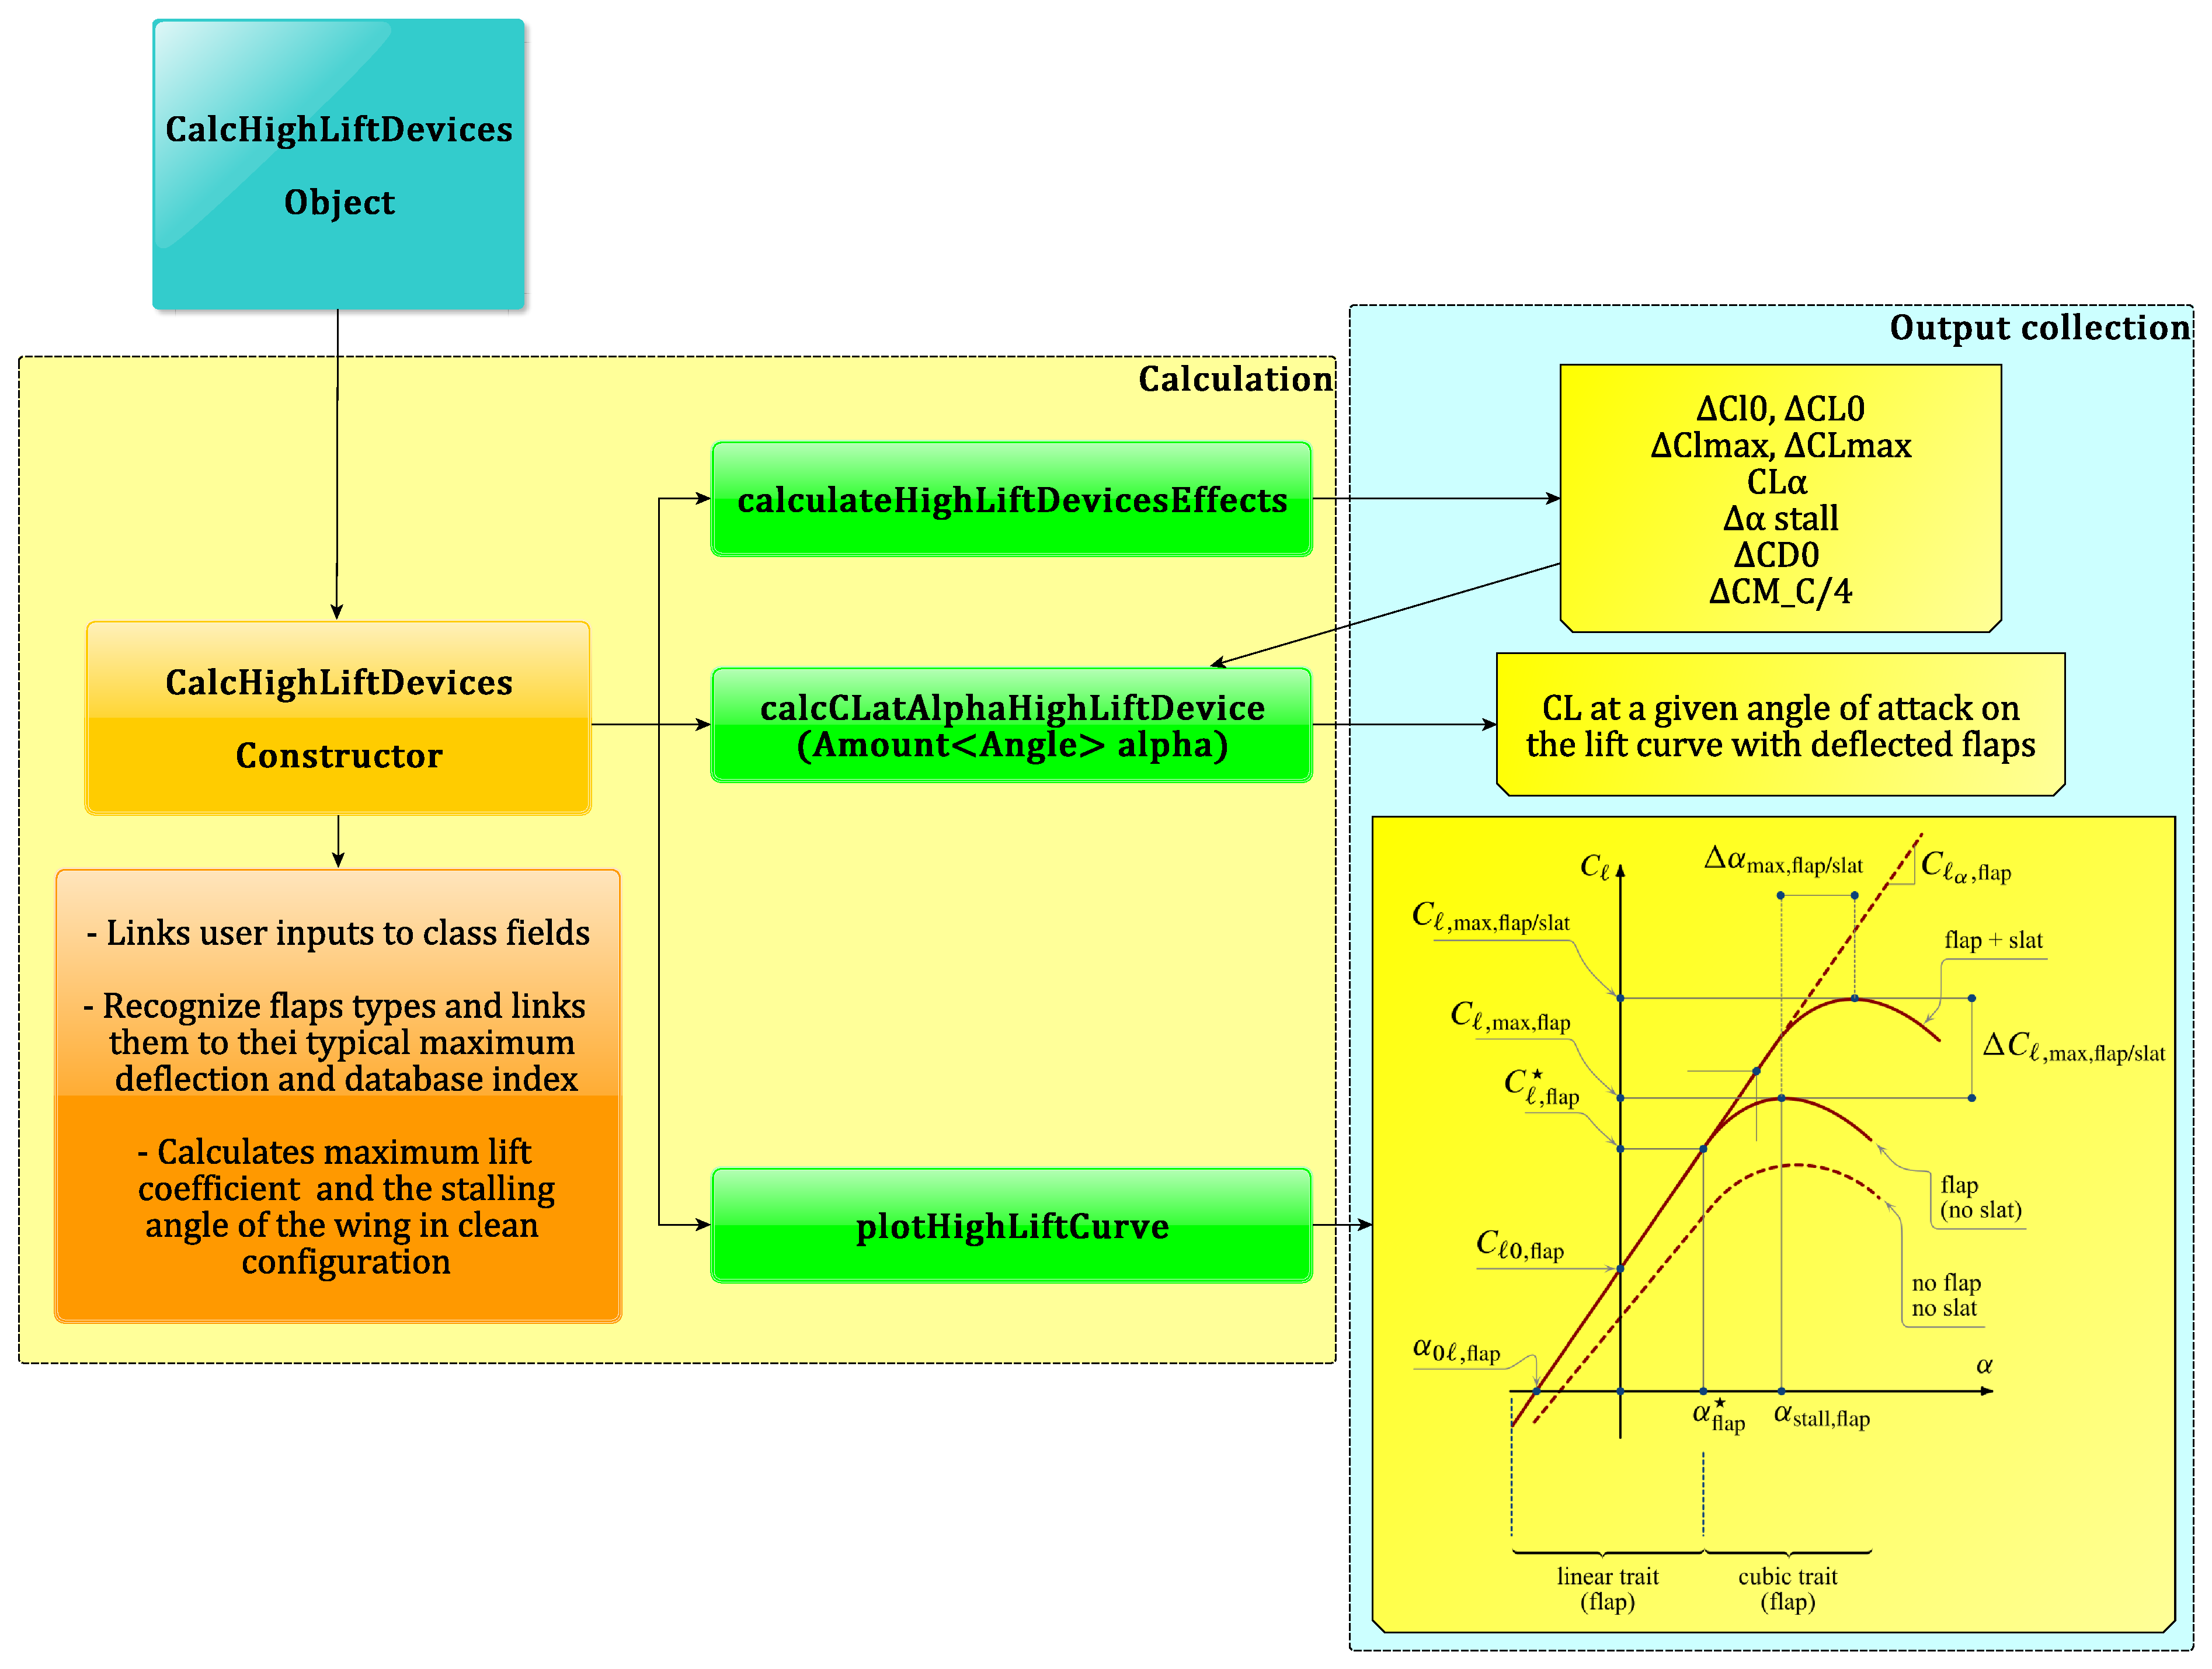
\includegraphics[keepaspectratio, width=0.78\paperwidth]{images/HighLiftDevices_Flowchart}
}
%
\begin{frame}{High Lift Devices Java class flowchart}
\end{frame}
\setbeamertemplate{background canvas}{ }
%
%-----------------------Frame 25------------------------------
\placelogotrue
\placebackgroundfalse
\begin{frame}{High Lift Devices Java class output}
\only<1>{
\begin{columns}[onlytextwidth,t]
\column{0.5\textwidth}
\Wider{
  \vspace*{-1.5cm}
\textbf{\textcolor{mygold}{ATR-72 @ Take-Off}}
\begin{itemize}
	\MyBullet 2 Single slotted flap
	\MyBullet $\frac{c_f}{c}=0.35$
	\MyBullet $\delta_f=\SI{20}{\degree}$
	\MyBullet $\eta_{\text{in, flap1}}=0.08;\ \eta_{\text{out, flap1}}=0.35$
	\MyBullet $\eta_{\text{in, flap2}}=0.35;\ \eta_{\text{out, flap2}}=0.8$
\end{itemize}
\vspace*{0.15cm}
\hspace*{0.15cm}
\scalebox{0.95}{
\begin{tabular}{|l||c|c|}
\hline
\textbf{ } & \textbf{No Flap} &  \textbf{Flap}\\
\hline\hline
\textbf{$\alpha_{\text{stall}}$} & $\SI{17.47}{\degree}$ & $\SI{15.54}{\degree}$\\
\textbf{$C_{L\text{max}}$} & 1.59 & 2.11\\
\textbf{$C_{L\text{star}}$} & 1.095 & 1.54\\
\textbf{$C_{L\alpha}$} (1/rad) & 5.19 & 5.24\\
\hline
\end{tabular}
}
}
\column{0.5\textwidth}
\WiderImages{
\begin{figure}
  \vspace*{-1.38cm}
  \hspace*{0.8cm}
\centering
    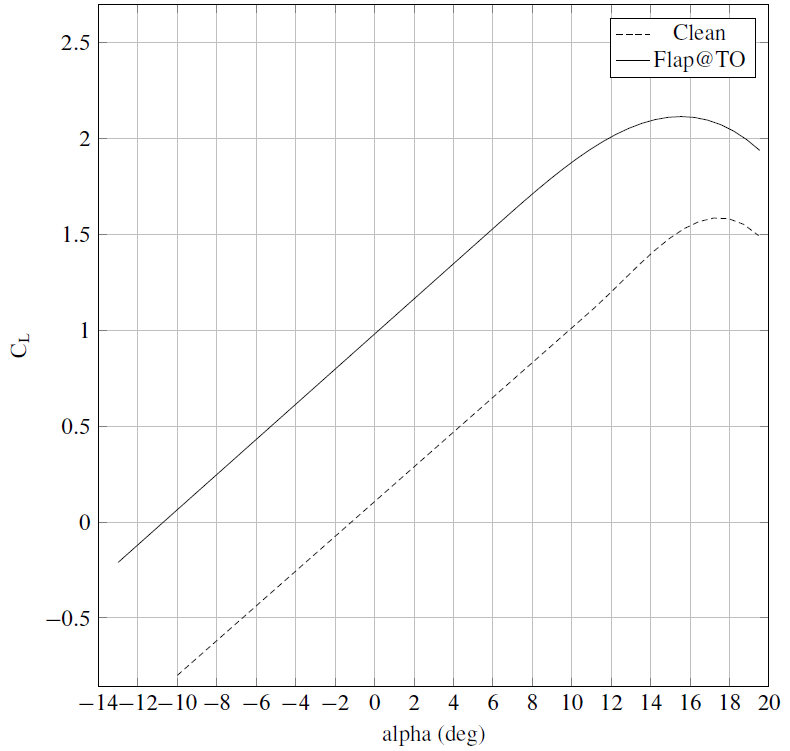
\includegraphics[keepaspectratio, width=0.5\paperwidth]{images/ATRFlapTO.PNG}
    \captionsetup{labelformat=empty}
\end{figure}
}
\end{columns}
}
\pause
\only<2>{
\begin{columns}[onlytextwidth,t]
\column{0.5\textwidth}
\Wider{
  \vspace*{-1cm}
\textbf{\textcolor{mygold}{B747-100B @ Landing}}
\begin{itemize}
	\MyBullet 2 Double slotted flap + 2 Slat
	\MyBullet $\frac{c_f}{c}=0.25;\quad \frac{c_s}{c}=0.15$
	\MyBullet $\delta_f=\left(\SI{20}{\degree}+\SI{25}{\degree}\right);\quad \delta_s=\SI{5}{\degree}$
	\MyBullet $\frac{c'}{c}_{\text{slat}}=1.1;\quad \frac{\text{LER}}{c}_{\text{slat}}=0.0097$
	\MyBullet $\eta_{\text{in, flap1}}=0.11;\ \eta_{\text{out, flap1}}=0.38$
	\MyBullet $\eta_{\text{in, flap2}}=0.38;\ \eta_{\text{out, flap2}}=0.72$
	\MyBullet $\eta_{\text{in, slat1}}=0.14;\ \eta_{\text{out, slat1}}=0.37$
	\MyBullet $\eta_{\text{in, slat2}}=0.42;\ \eta_{\text{out, slat}}=0.9$
\end{itemize}
\vspace*{0.15cm}
\hspace*{1.55cm}
\scalebox{0.8}{
\begin{tabular}{|l||c|c|}
\hline
\textbf{ } & \textbf{No Flap} &  \textbf{Flap}\\
\hline\hline
\textbf{$\alpha_{\text{stall}}$} & $\SI{23.23}{\degree}$ & $\SI{21.94}{\degree}$\\
\textbf{$C_{L\text{max}}$} & 1.47 & 2.99\\
\textbf{$C_{L\text{star}}$} & 0.83 & 2.35\\
\textbf{$C_{L\alpha}$} (1/rad) & 4.089 & 4.12\\
\hline
\end{tabular}
}
}
\column{0.5\textwidth}
\WiderImages{
\begin{figure}
  \vspace*{-1.1cm}
  \hspace*{1.16cm}
\centering
    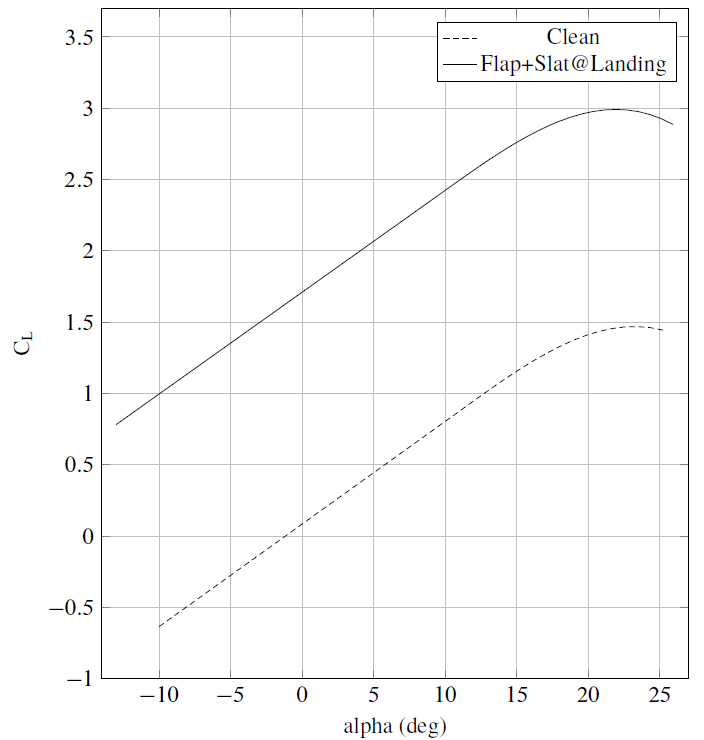
\includegraphics[keepaspectratio, width=0.48\paperwidth]{images/B747FlapSlatLand.PNG}
    \captionsetup{labelformat=empty}
\end{figure}
}
\end{columns}
}
\end{frame}
%
%----------------Current table of contents--------------------
\placelogotrue
\placebackgroundfalse
\begin{frame}{Table of Contents}
\section{Take-Off and Landing classes}
\vspace*{-1cm}
\tableofcontents[currentsection]
\subsection{}
\end{frame}
%
%-----------------------Frame 26------------------------------
\placelogotrue
\placebackgroundfalse
\begin{frame}{ODE set for the AOE take-off distance calculation}
\Wider{
\only<1>{
\vspace*{0.8cm}
\textcolor{mygold}{State space representation $\qquad\dot{\vec{x}} = \vec{f}\big(\, \vec{x}\,;\,u \,\big)$}
\vspace*{-0.3cm}
\begin{align*}
\scalebox{0.8}{$
    \left\{\begin{array}{c}\dot{s}\\[2pt] \dot{V} \\[2pt] \dot{\gamma} \\[2pt] \dot{h} \end{array}\right\}
= 
    \left\{\begin{array}{l}
       f_1 \big(\, s,\, V,\, \gamma,\, h \,; \, \alpha \big) \\[4pt]
       f_2 \big(\, s,\, V,\, \gamma,\, h \,; \, \alpha \big) \\[4pt]
       f_3 \big(\, s,\, V,\, \gamma,\, h \,; \, \alpha \big) \\[4pt]
       f_4 \big(\, s,\, V,\, \gamma,\, h \,; \, \alpha \big)
    \end{array}\right\}
\quad
    \text{with}\quad
   \left\{\begin{array}{l} x_1 = s\\[2pt] x_2 = V \\[2pt] x_3 = \gamma \\[2pt] x_4 = h \end{array}\right\}
\quad
    \text{and}\quad
    u = \alpha
$}
\end{align*}
\vspace*{-0.5cm}
\begin{itemize}
	\MyBullet \scalebox{0.8}{$f_1 \big(\, \vec{x}\,,\,u \,\big) =  x_2$}
	\MyBullet \scalebox{0.8}{$f_2 \big(\, \vec{x}\,,\,u \,\big) =
  \dfrac{g}{W}
    \left\{
      \begin{array}{l@{\rule{2em}{0pt}}l} 
         \scalebox{0.8}{$
         T(x_2) - D(x_2,u) - \mu \big[ W - L(x_2,u) \big]$}
          & \text{if} \;\, \mathcal{S}(x_2 , u) < 1
        \\[1em]
         \scalebox{0.8}{$
         T(x_2) \cos u - D(x_2,u) - W \sin x_3$}
          & \text{if} \;\, \mathcal{S}(x_2 , u) \geq 1
      \end{array}\right\}$}
	\MyBullet \scalebox{0.8}{$f_3 \big(\, \vec{x}\,,\,u \,\big) =
  \dfrac{g}{W\,x_2}
   \left\{
      \begin{array}{l@{\rule{2em}{0pt}}l} 
       \scalebox{0.8}{$
        0 $}
          & \text{if} \;\, \mathcal{S}(x_2 , u) < 1
        \\[1em]
         \scalebox{0.8}{$
        L(x_2,u) + T(x_2)\sin u - W \cos x_3$}
          & \text{if} \;\, \mathcal{S}(x_2 , u) \geq 1
      \end{array}
    \right\}$}
	\MyBullet \scalebox{0.8}{$f_4 \big(\, \vec{x}\,,\,u \,\big) =  x_2 \, \sin x_3$}
\end{itemize}
\begin{center}
	\scalebox{0.8}{$\mathcal{S}(x_2 , u) = \dfrac{L(x_2,u)}{W \cos x_3}$}
\end{center}
}
\only<2>{
\vspace*{0.2cm}
\textcolor{mygold}{State vector and input $\quad {\vec{x}} = \left\{x_1 = s;\ x_2 = V;\ x_3 = \gamma;\ x_4 = h\right\};\ u=\alpha$}
\begin{columns}[onlytextwidth,t]
\column{0.7\textwidth}
\begin{itemize}
	\vspace*{-0.3cm}
	\MyBullet $T(x_2)$ is read from the engine database related to the take-off setting.
	\MyBullet $D(x_2,u) = \dfrac{1}{2} \, \rho \, \big( x_2 + V_{\text{w}}\cos x_3 \big)^2 \,S \, C_D\big( u \big)$ 
	\begin{itemize}
	\vspace*{0.cm}
		\MyBullet $C_D\big(u\big) = C_{D0} + \left(\text{$\Delta$}C_{D0}\right)_{\text{flap}+\text{lg}} +  K_g\ \dfrac{C_L^2}{\pi\AR e}$
		\begin{itemize}
		\vspace*{0.2cm}
			\MyBullet $K_g=-622.44x^5+624.46x^4-255.24x^3+47.105x^2-0.6378x+0.0055$
		\end{itemize}
		\vspace*{0.2cm}
	\end{itemize}
	\MyBullet $L(x_2,u) = \dfrac{1}{2} \, \rho \, \big( x_2 + V_{\text{w}}\cos x_3 \big)^2 \,S \, C_L\big( u \big)$
	\begin{itemize}
	\vspace*{0.1cm}
		\MyBullet $C_L\big(u\big)$ is the one from the lift curve with flaps, and eventually slats, deflected.
	\end{itemize}
\end{itemize}
\column{0.3\textwidth}
\WiderImages{
\begin{figure}
  \vspace*{0.5cm}
  \hspace*{-0.5cm}
\centering
    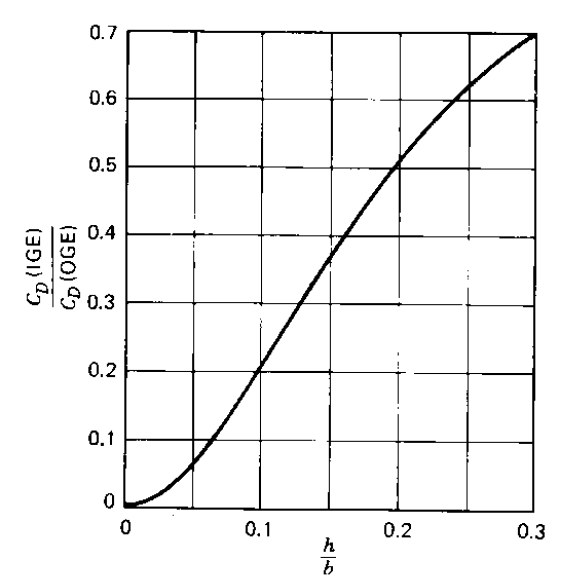
\includegraphics[keepaspectratio, width=0.79\textwidth]{images/McCormickGroundEffect.PNG}
    \captionsetup{labelformat=empty}
\end{figure}
}
\end{columns}
}
\only<3>{
\begin{columns}[onlytextwidth,t]
\column{0.4\textwidth}
\vspace*{-6.5cm}
\begin{align*}
\scalebox{0.8}{$
u (t) =
    \left\{
      \begin{array}{l@{\rule{2em}{0pt}}l} 
       \alert{\alpha_{\text{g}}}
          & \text{if} \;\, t < t_{\text{Rot}}
        \\[1em]
        \alpha_1(t)
          & \text{if} \;\, t \geq t_{\text{Rot}}
      \end{array}
    \right\}$}
\end{align*}
\begin{align*}
	\alpha_1(t) = \dot\alpha(t)\ dt
\end{align*}
\begin{align*}
\scalebox{0.8}{$
\dot\alpha (t) =
    \left\{
      \begin{array}{l@{\rule{2em}{0pt}}l} 
      \alert{\dot\alpha_0}\ \left(1-\alert{k_\alpha}\ \alpha\right)
          & \text{if} \;\, t_{\text{Rot}} \leq t < t_{\text{Hold}}
        \\[1em]
        0
          & \text{if} \;\, t_{\text{Hold}} \leq t < t_{\text{Hold}}+\text{$\Delta$}t_{\text{Hold}}
          \\[1em]
	\alert{\dot\alpha_{\text{red}}}
          & \text{if} \;\,  t_{\text{Hold}}+\text{$\Delta$}t_{\text{Hold}} \leq t < t_{\text{climb}}
          \\[1em]
        0
          & \text{if} \;\,  t \geq t_{\text{climb}} 
      \end{array}
    \right\}$}
\end{align*}
\column{0.4\textwidth}
\centering
\hspace{-0.5cm}
    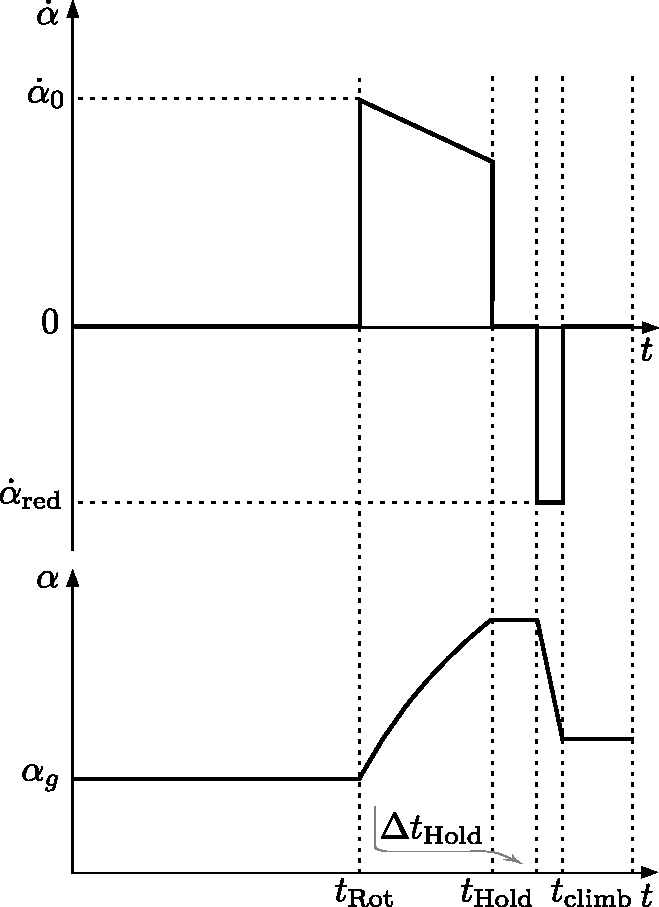
\includegraphics[keepaspectratio, width=0.9\textwidth]{images/AlphaInputTakeOff}
    \captionsetup{labelformat=empty}
\end{columns}
}
}
\end{frame}
%
%-----------------------Frame 27------------------------------
\placelogotrue
\placebackgroundfalse
\begin{frame}{ODE set modification for the take-off in OEI condition}
\Wider{
\vspace*{0.2cm}
\textcolor{mygold}{OEI continued take-off}
\begin{itemize}
	\MyBullet There is a discontinuity in thrust at a specific failure speed $V_{ef}$.
	\MyBullet $T(x_2)$ is still read from the database but considering a number of engines reduced by one from the time $t_{ef}$ at which the engine failure occurs.
\end{itemize}
\textcolor{mygold}{OEI aborted take-off}
\begin{itemize}
	\MyBullet The take-off run, up to the engine failure speed $V_{ef}$, is the same as the continued take-off one.
	\MyBullet The pilot reacts at a time $t_{\text{act}}$ (generally $\SI{3}{\second}$ after $t_{ef}$) setting $T(x_2)$ to 0 and activating brakes. The equation $f_2$ changes in the following.
\end{itemize}
\begin{align*}
	f_2 \big(\, \vec{x}\,,\,u \,\big) =\frac{g}{W}\ \big\{ - D(x_2,u) - \mu_{\text{brakes}} \big[ W - L(x_2,u) \big]\big\} 
\end{align*}
}
\end{frame}
%
%-----------------------Frame 28------------------------------
\placelogotrue
\placebackgroundfalse
\begin{frame}{Landing distance calculation}
\Wider{
\only<1>{
\vspace*{1cm}
\textbf{\textcolor{mygold}{Air run}}
\begin{itemize}
	\MyBullet $\big[n=1.2$, $V_{\text{Flare}}=1.23\ V_s\big]\ \textcolor{mygold}{\rightarrow\ R=\dfrac{V^2}{g\left(n-1\right)}=\dfrac{V_{\text{Flare}}^2}{0.2\ g}}$
	\MyBullet $\big[\theta_a\approx\SI{2}{\degree}\div\SI{3}{\degree}\big]\ \textcolor{mygold}{\rightarrow\ h_{\text{Flare}}=R\left(1-\cos\theta_a\right)}$
	\MyBullet $\big[\theta_a$, $R$, $h_{\text{Flare}}\big]\ \alert{\rightarrow\ S_A=\dfrac{50-h_{\text{Flare}}}{\tan\theta_a}; \quad S_{\text{Flare}}=R\sin\theta_a}$
\end{itemize}
\begin{center}
	\vspace*{-0.5cm}
	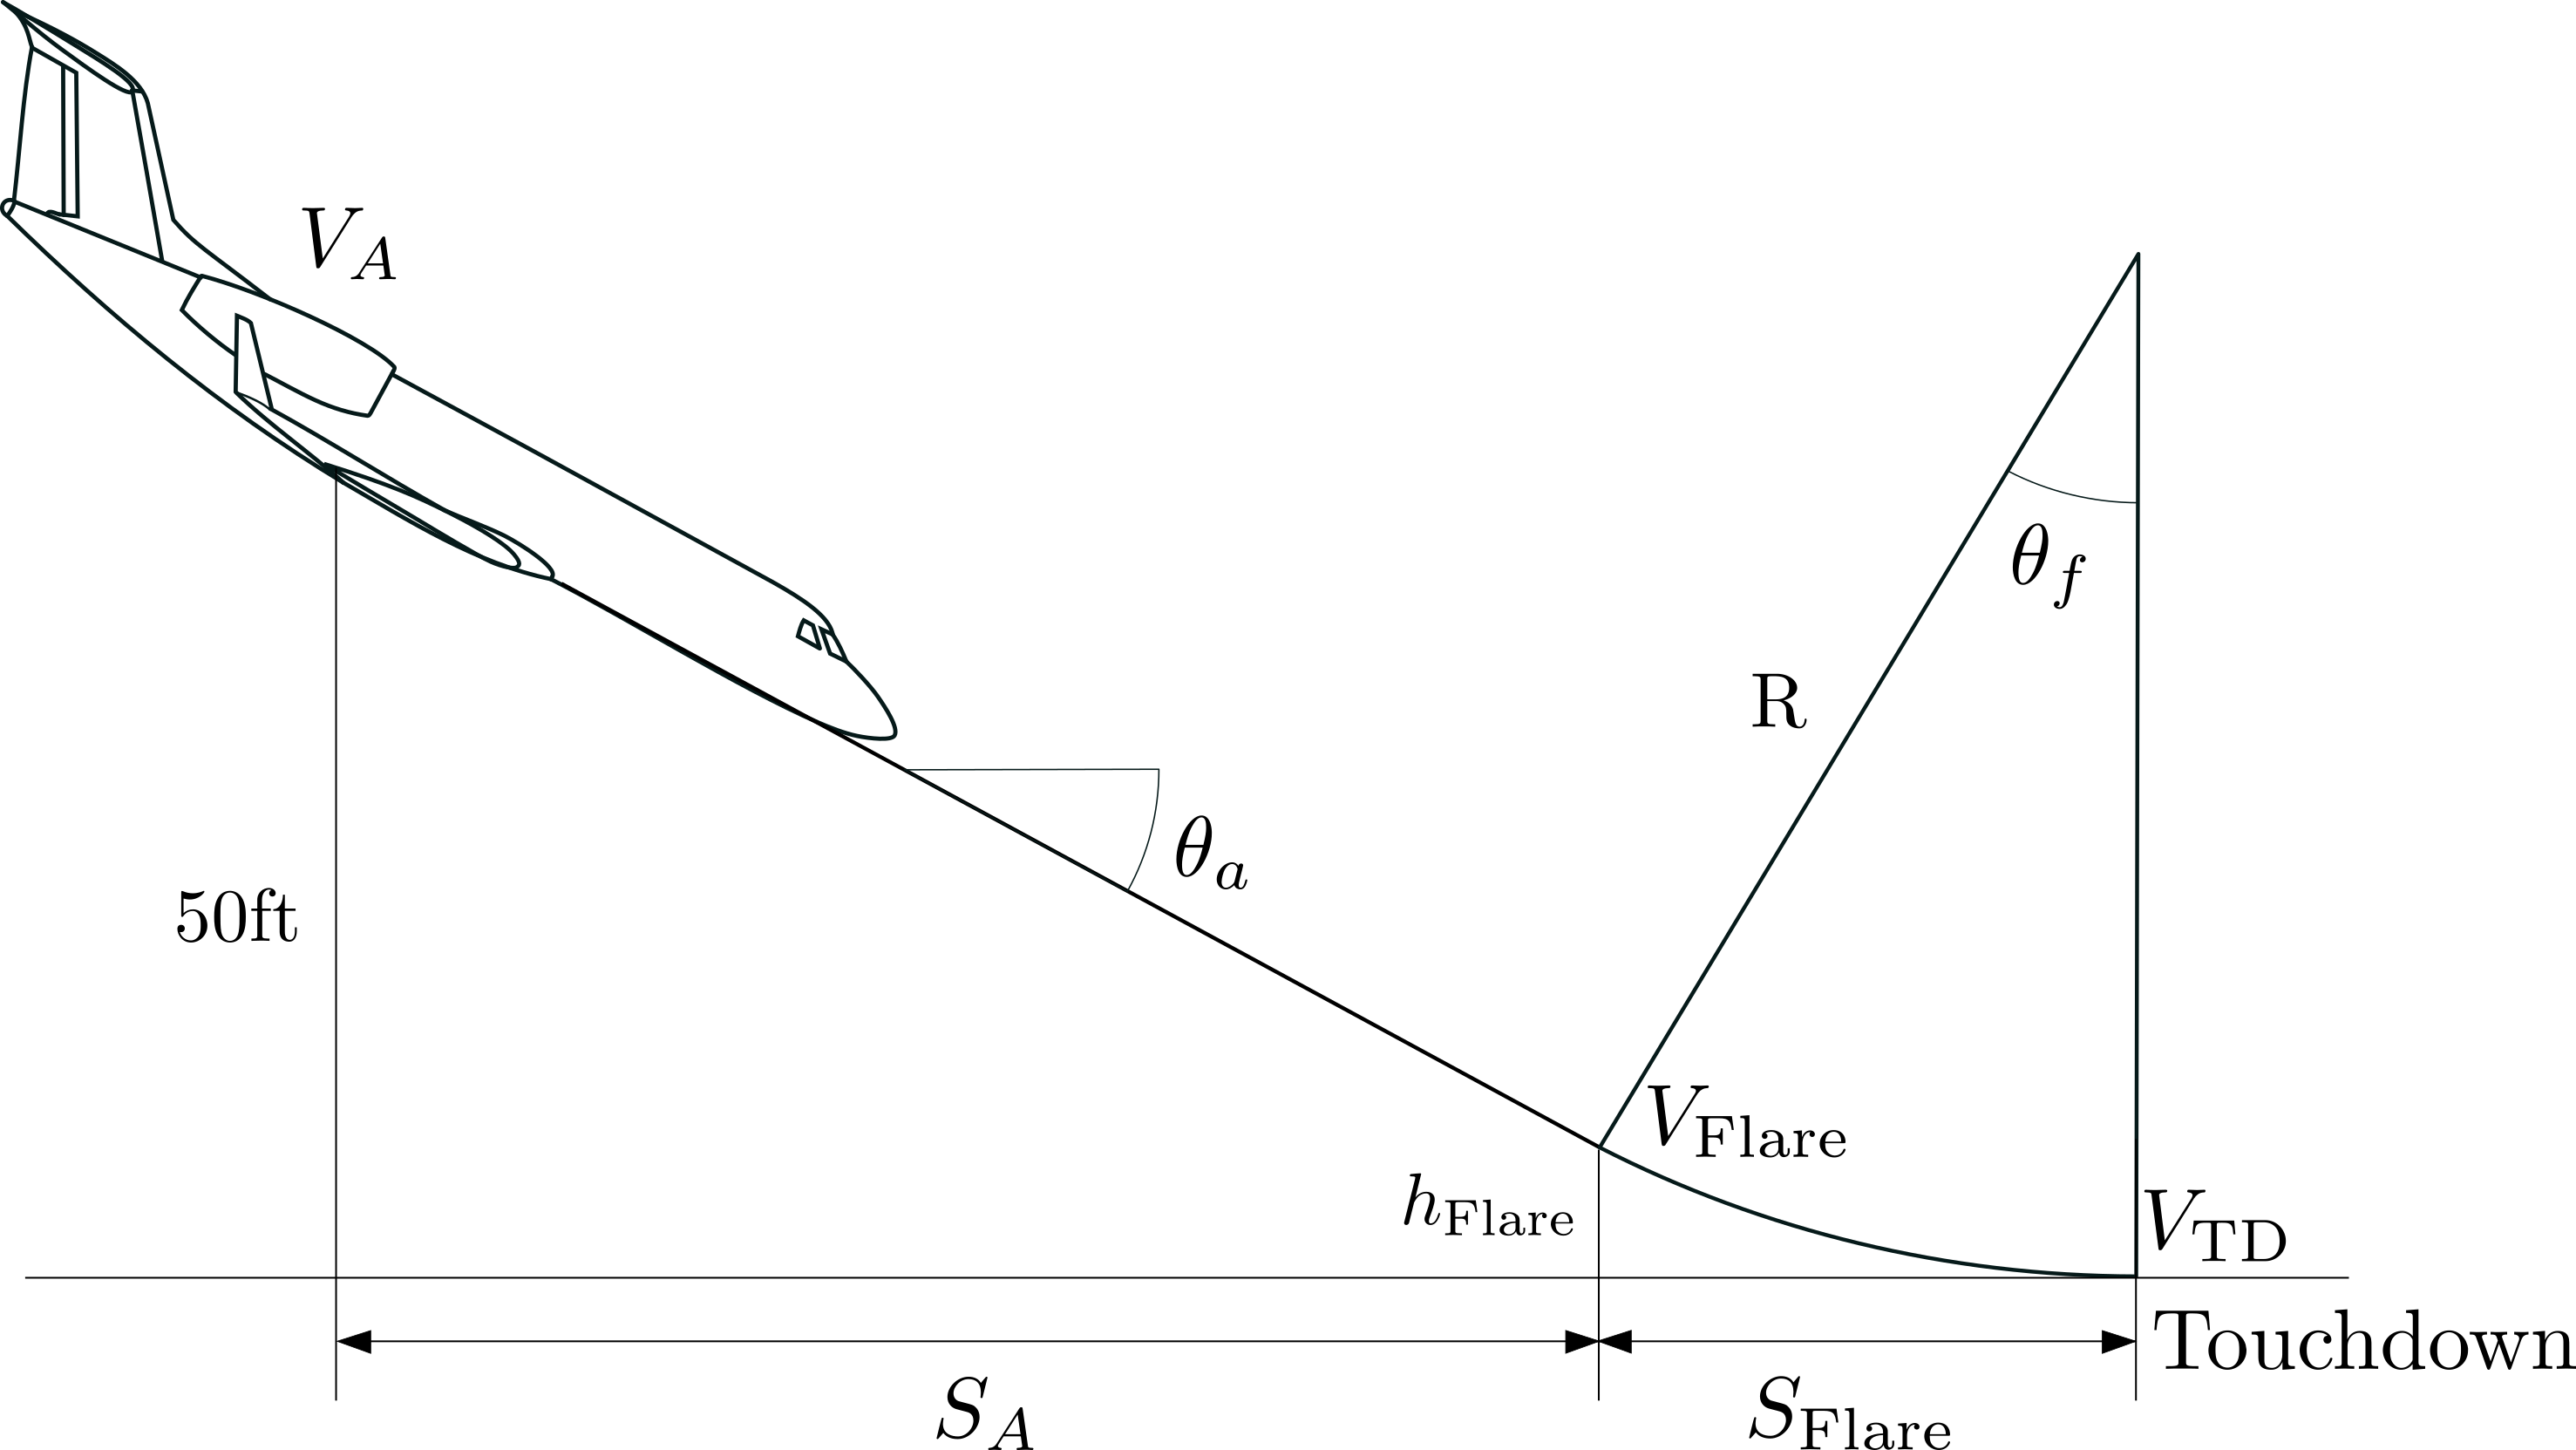
\includegraphics[keepaspectratio, width=0.6\textwidth]{images/LandingAirborne}
\end{center}
}
\only<2>{
\textbf{\textcolor{mygold}{Ground run}}
\begin{align*}
\scalebox{0.9}{$
    \left\{\begin{array}{c}\dot{s}\\[2pt] \dot{V}\end{array}\right\}
= 
    \left\{\begin{array}{l}
       f_1 \big(\, s,\, V\big) \\[4pt]
       f_2 \big(\, s,\, V\big) \\
    \end{array}\right\}
\quad
    \text{with}\quad
   \left\{\begin{array}{l} x_1 = s\\[2pt] x_2 = V\end{array}\right\}
$}
\end{align*}
\vspace*{-0.5cm}
\begin{itemize}
	\MyBullet \scalebox{0.9}{$f_1 \big(\, \vec{x}\,,\,u \,\big) =  x_2$}
	\MyBullet \scalebox{0.9}{$f_2 \big(\, \vec{x}\,\big) =
  \frac{g}{W}
    \left\{
      \begin{array}{l@{\rule{2em}{0pt}}l} 
        -T_{\text{Rev}}(x_2) - D(x_2) - \mu \big[ W - L(x_2) \big]
          & \text{if} \;\, t \leq t_{\text{fr}}
        \\[1em]
	-T_{\text{Rev}}(x_2) - D(x_2) - \mu_{\text{brakes}} \big[ W - L(x_2) \big]
          & \text{if} \;\, t > t_{\text{fr}}
      \end{array}
    \right\}$}
\end{itemize}
\vspace*{0.5cm}
\textcolor{mygold}{$t_{fr}$} is related to the end of the \textcolor{mygold}{\emph{free-roll distance}} (which represents the distance covered while the pilot reduces the power to idle, retracts the flaps, deploys the spoilers, and applies the brakes) and it’s set at \textcolor{mygold}{$\SI{3}{\second}$}.
}
}
\end{frame}
%
%-----------------------Frame 29------------------------------
\placelogotrue
\placebackgroundfalse
\begin{frame}{Take-Off Java class flowchart}
\vspace*{-0.35cm}
	\begin{center}
		\rule{-0.11in}{0in}%
		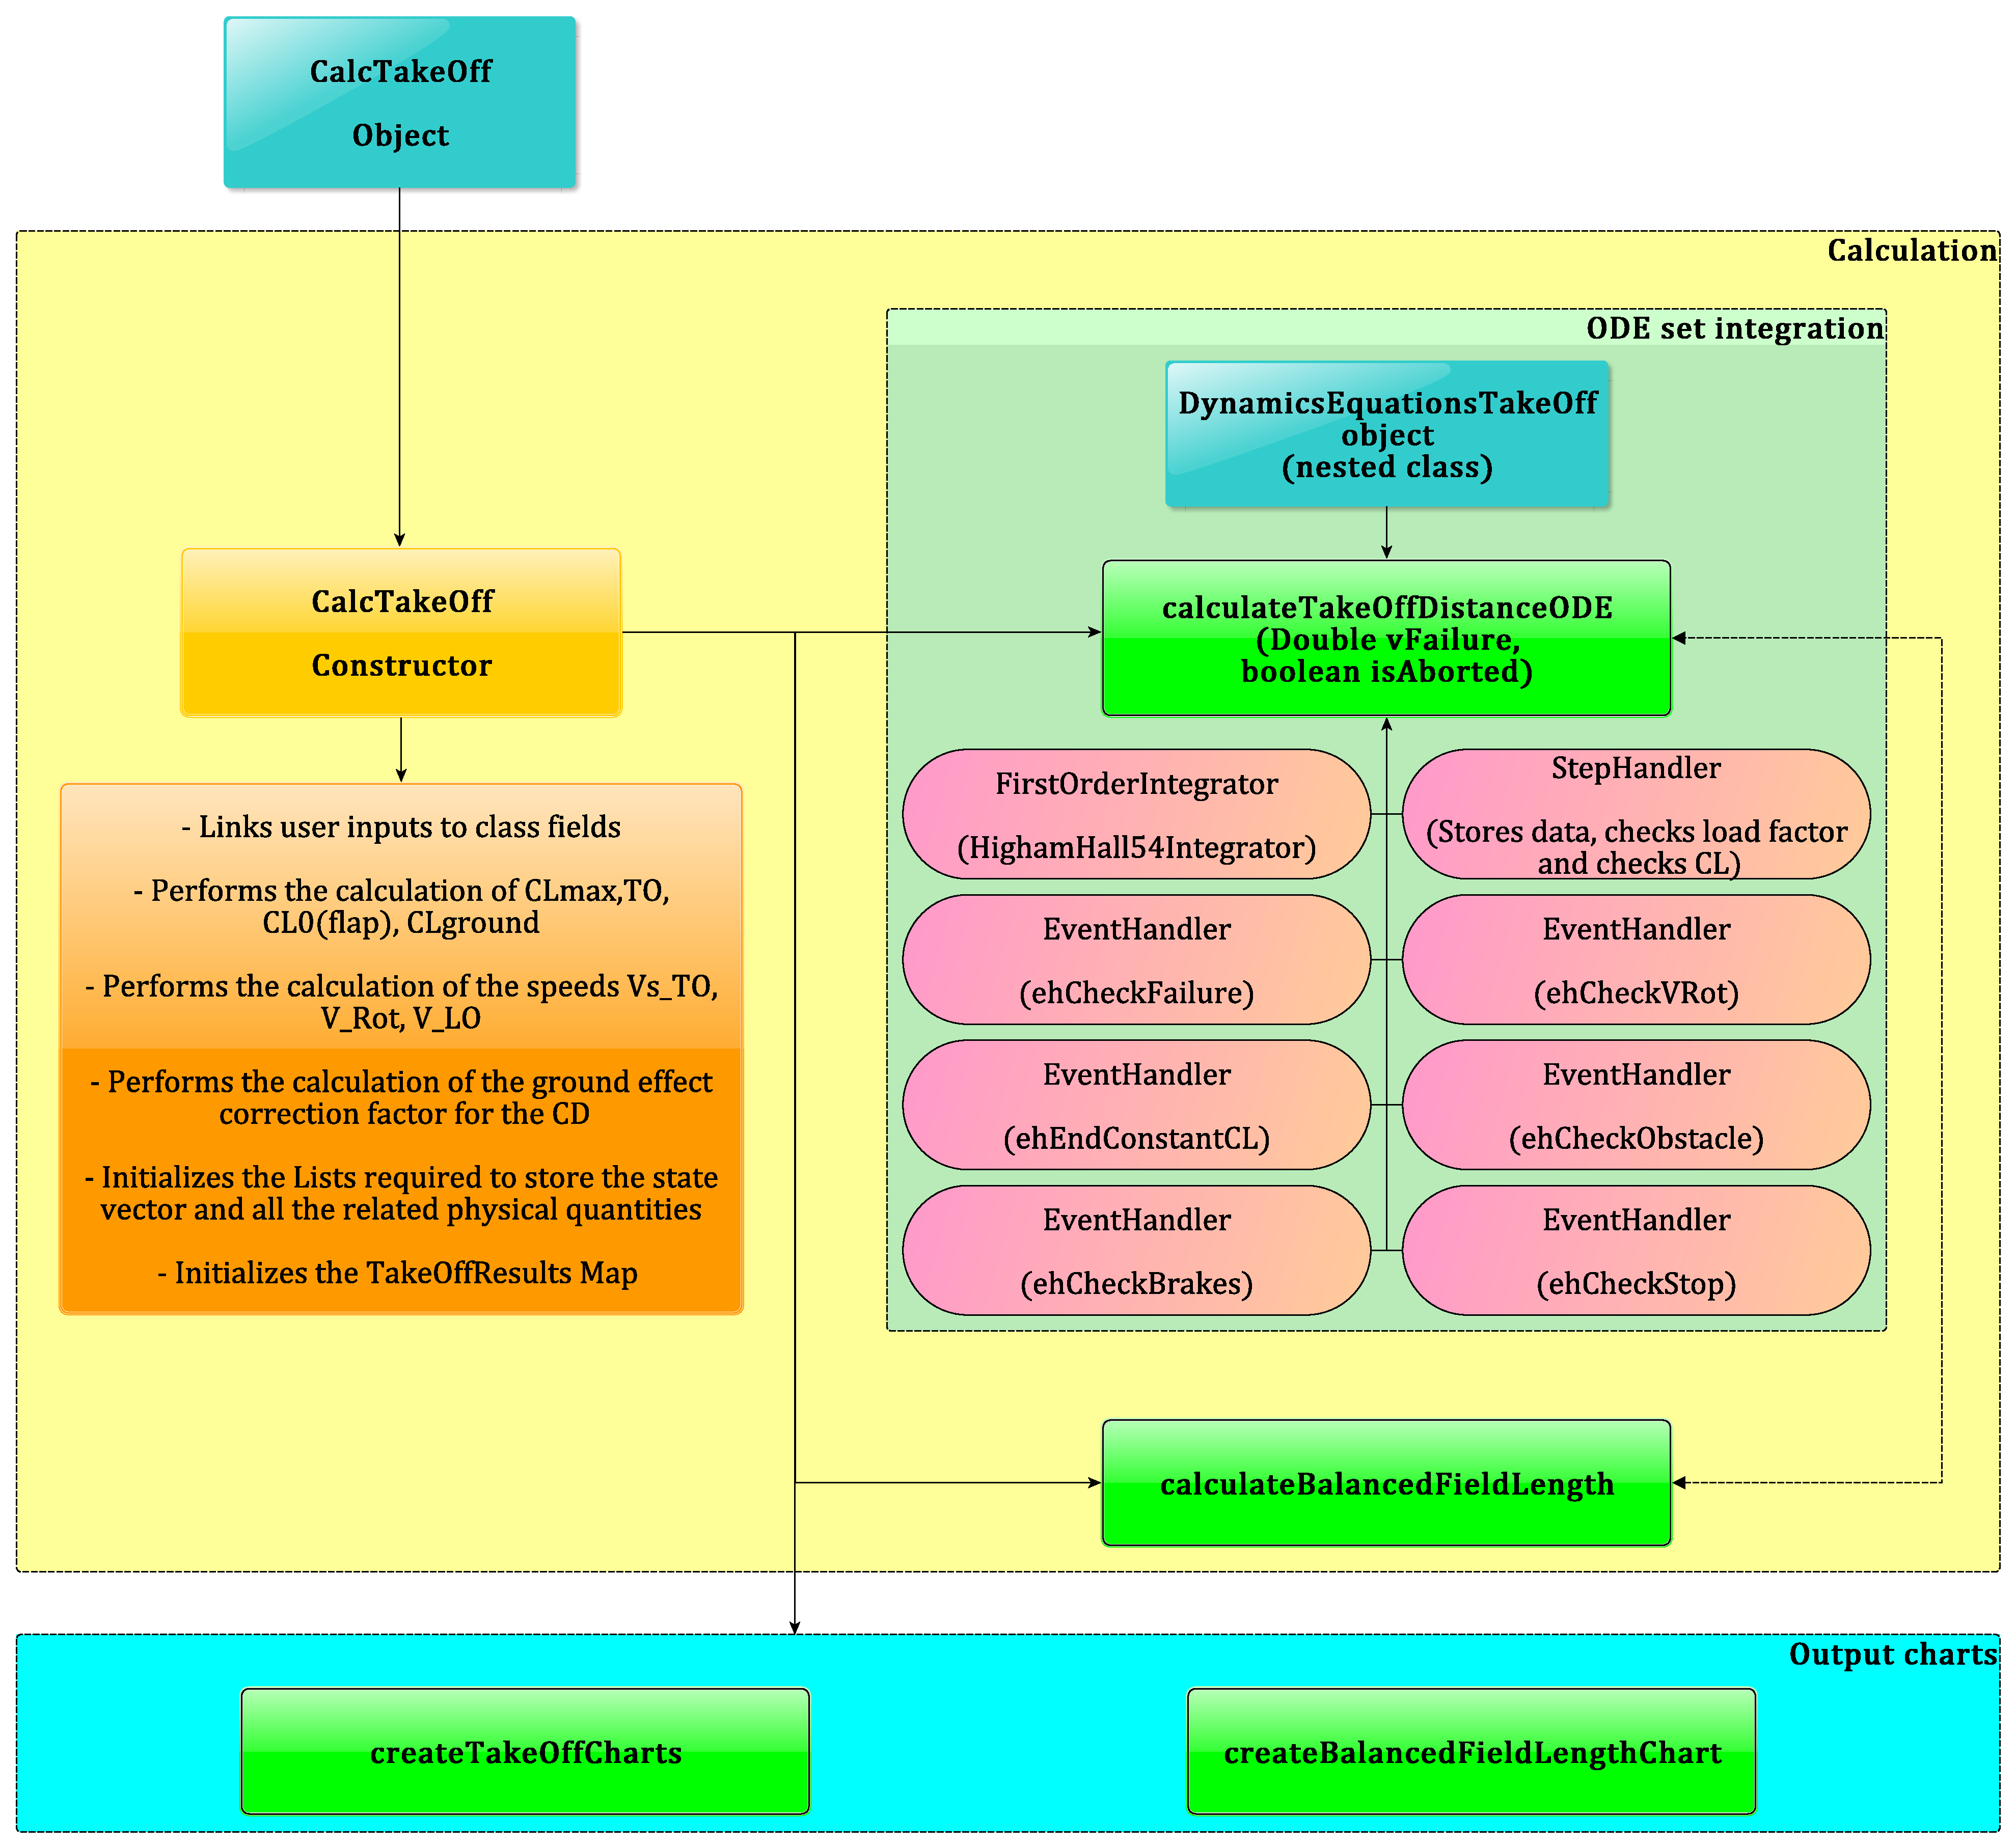
\includegraphics[keepaspectratio, width=0.79\textwidth]{images/TakeOff_Flowchart}
	\end{center}
\end{frame}
%
%-----------------------Frame 30------------------------------
\placelogotrue
\placebackgroundfalse
%
\setbeamertemplate{background canvas}{
    \rule{0in}{3.65in}%
    \rule{0.5in}{0in}%
    \centering
    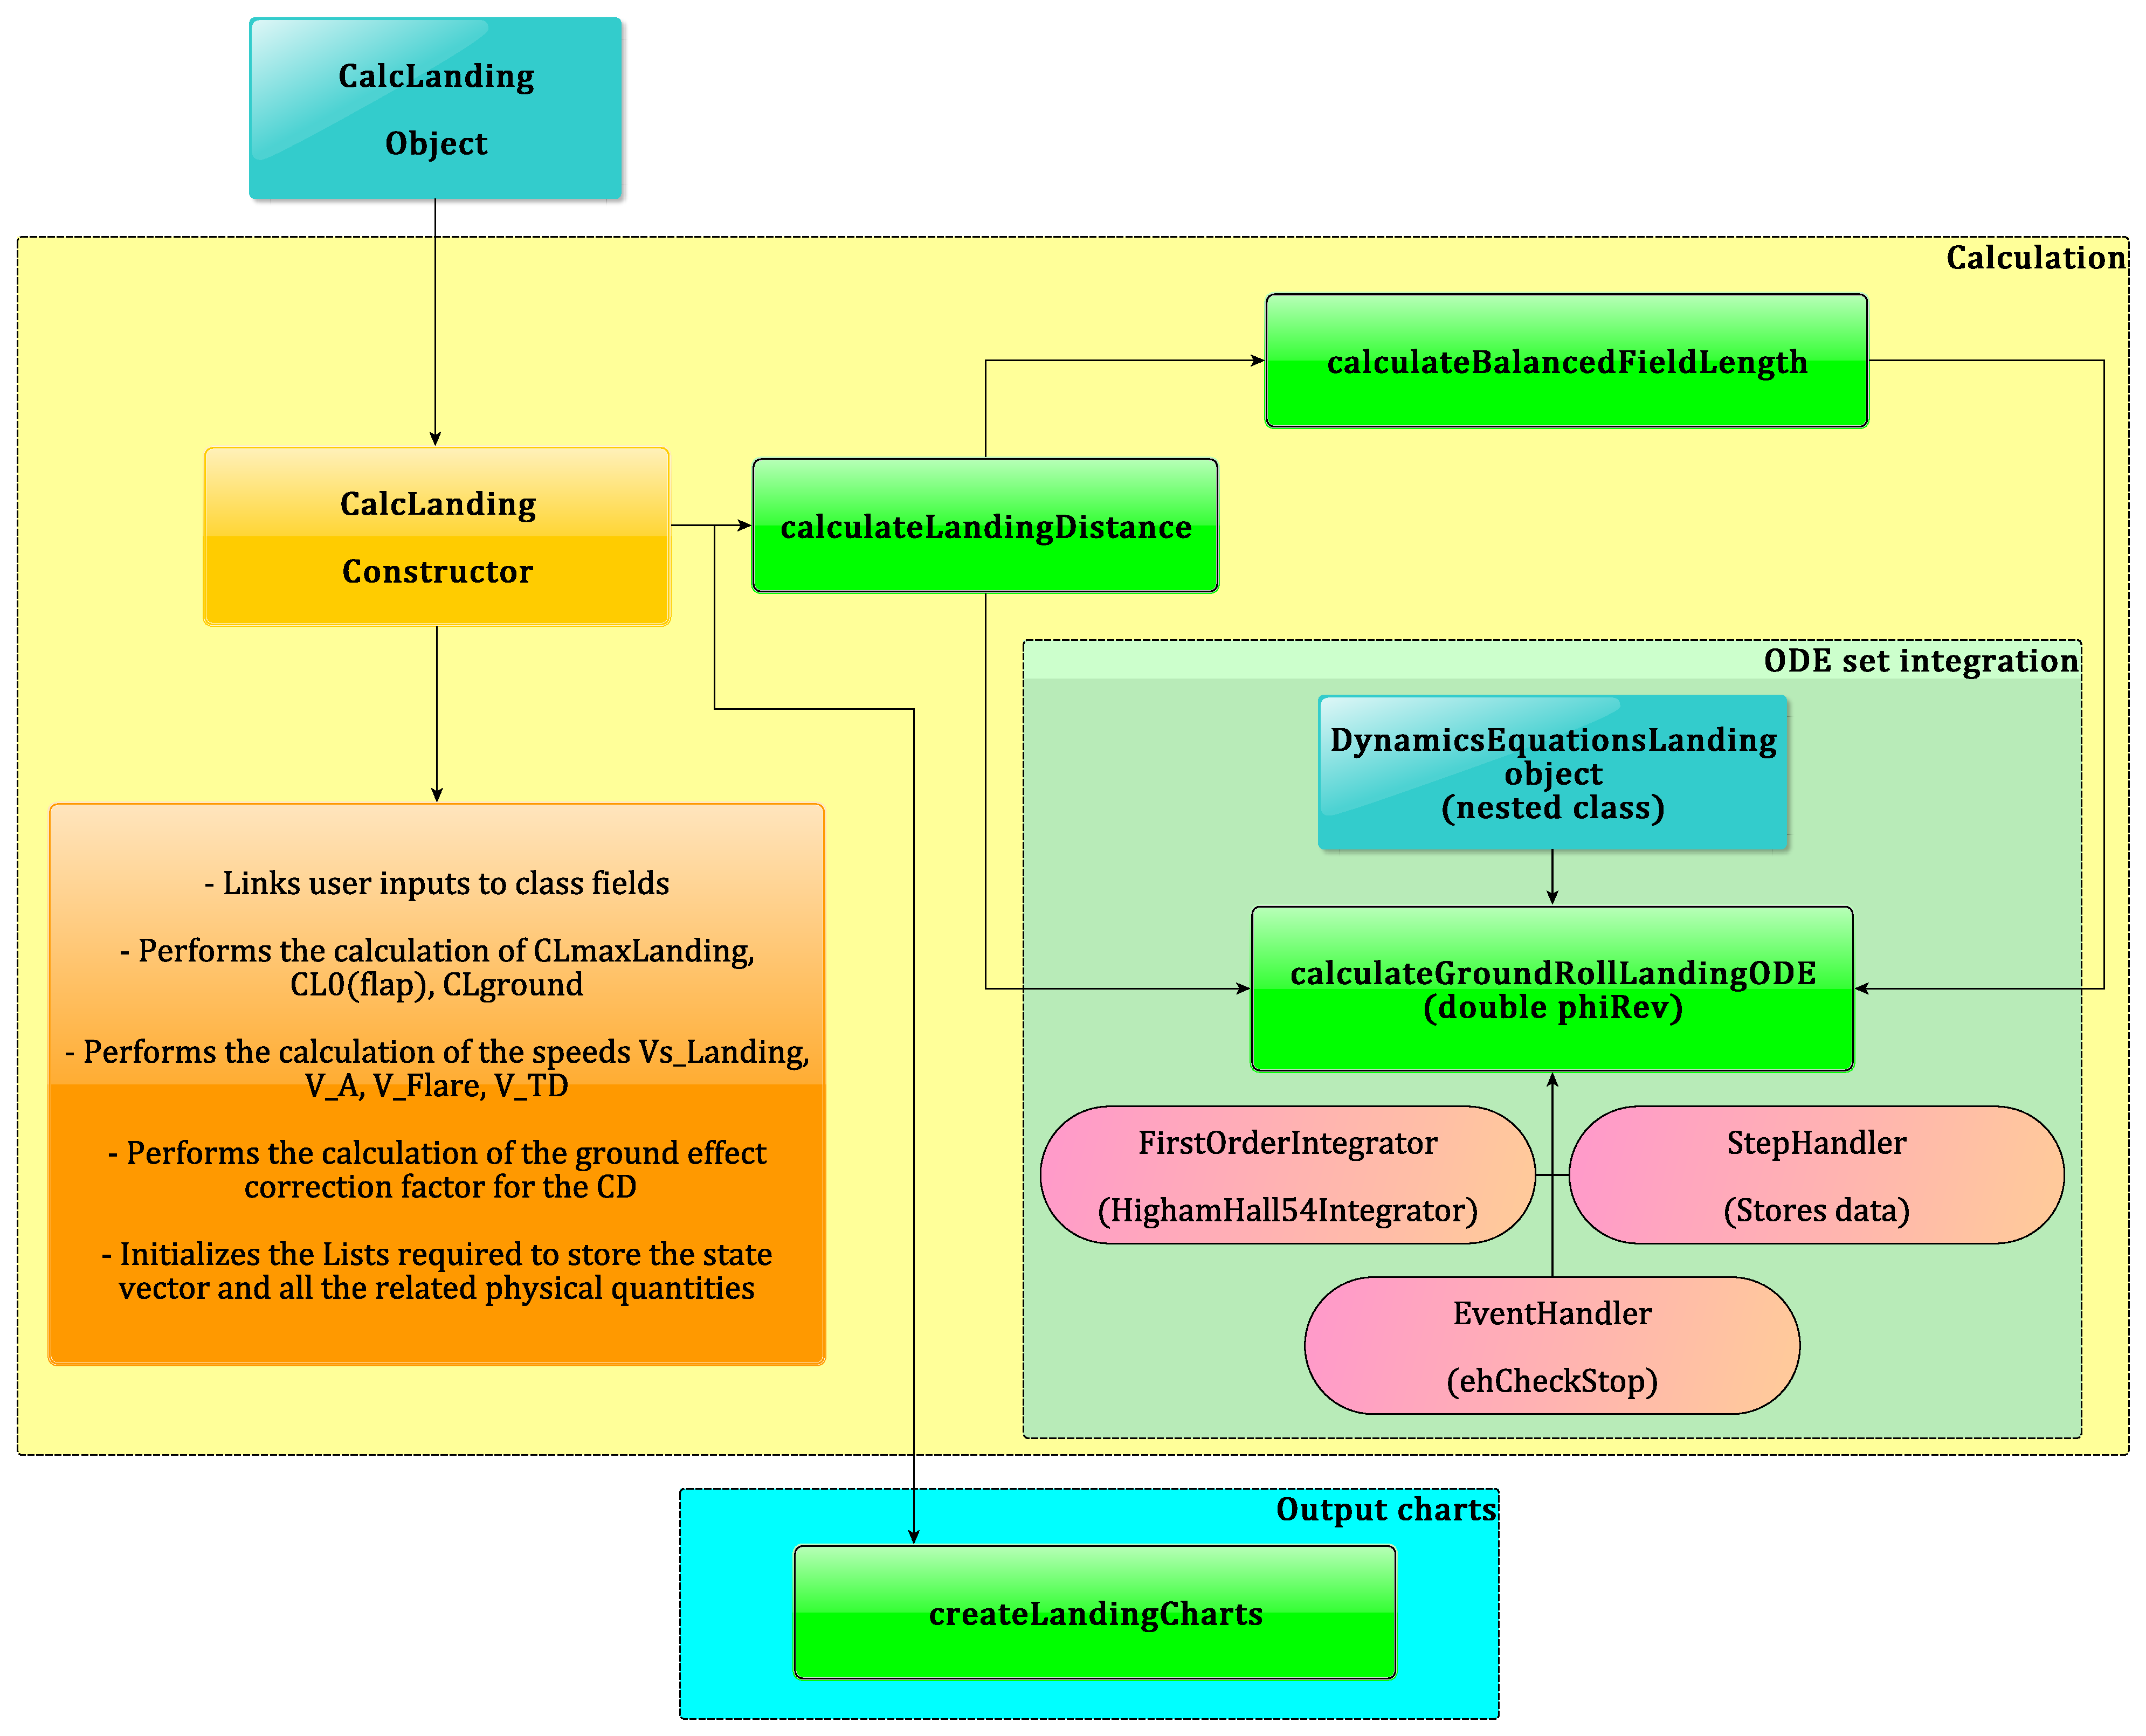
\includegraphics[keepaspectratio, width=0.9\textwidth]{images/Landing_Flowchart}
}
%
\begin{frame}{Landing Java class flowchart}
\end{frame}
%
\setbeamertemplate{background canvas}{ }
%
\end{document}